% DOCX paragraph 828
\chapter{The First Image Of A Black Hole}\label{ch:07}

% DOCX paragraph 829

% DOCX paragraph 832
So far, we have discussed in detail the properties of black holes and the intellectual
challenges these objects pose. Now it is time to present a recent scientific achievement
of great importance, which I have been fortunate and privileged to participate in as one
of the 13 members of the Executive Committee of the Event Horizon
Telescope\index{Event Horizon Telescope} (EHT) Collaboration.

% DOCX paragraph 833
\begin{figure}[htbp]
\centering
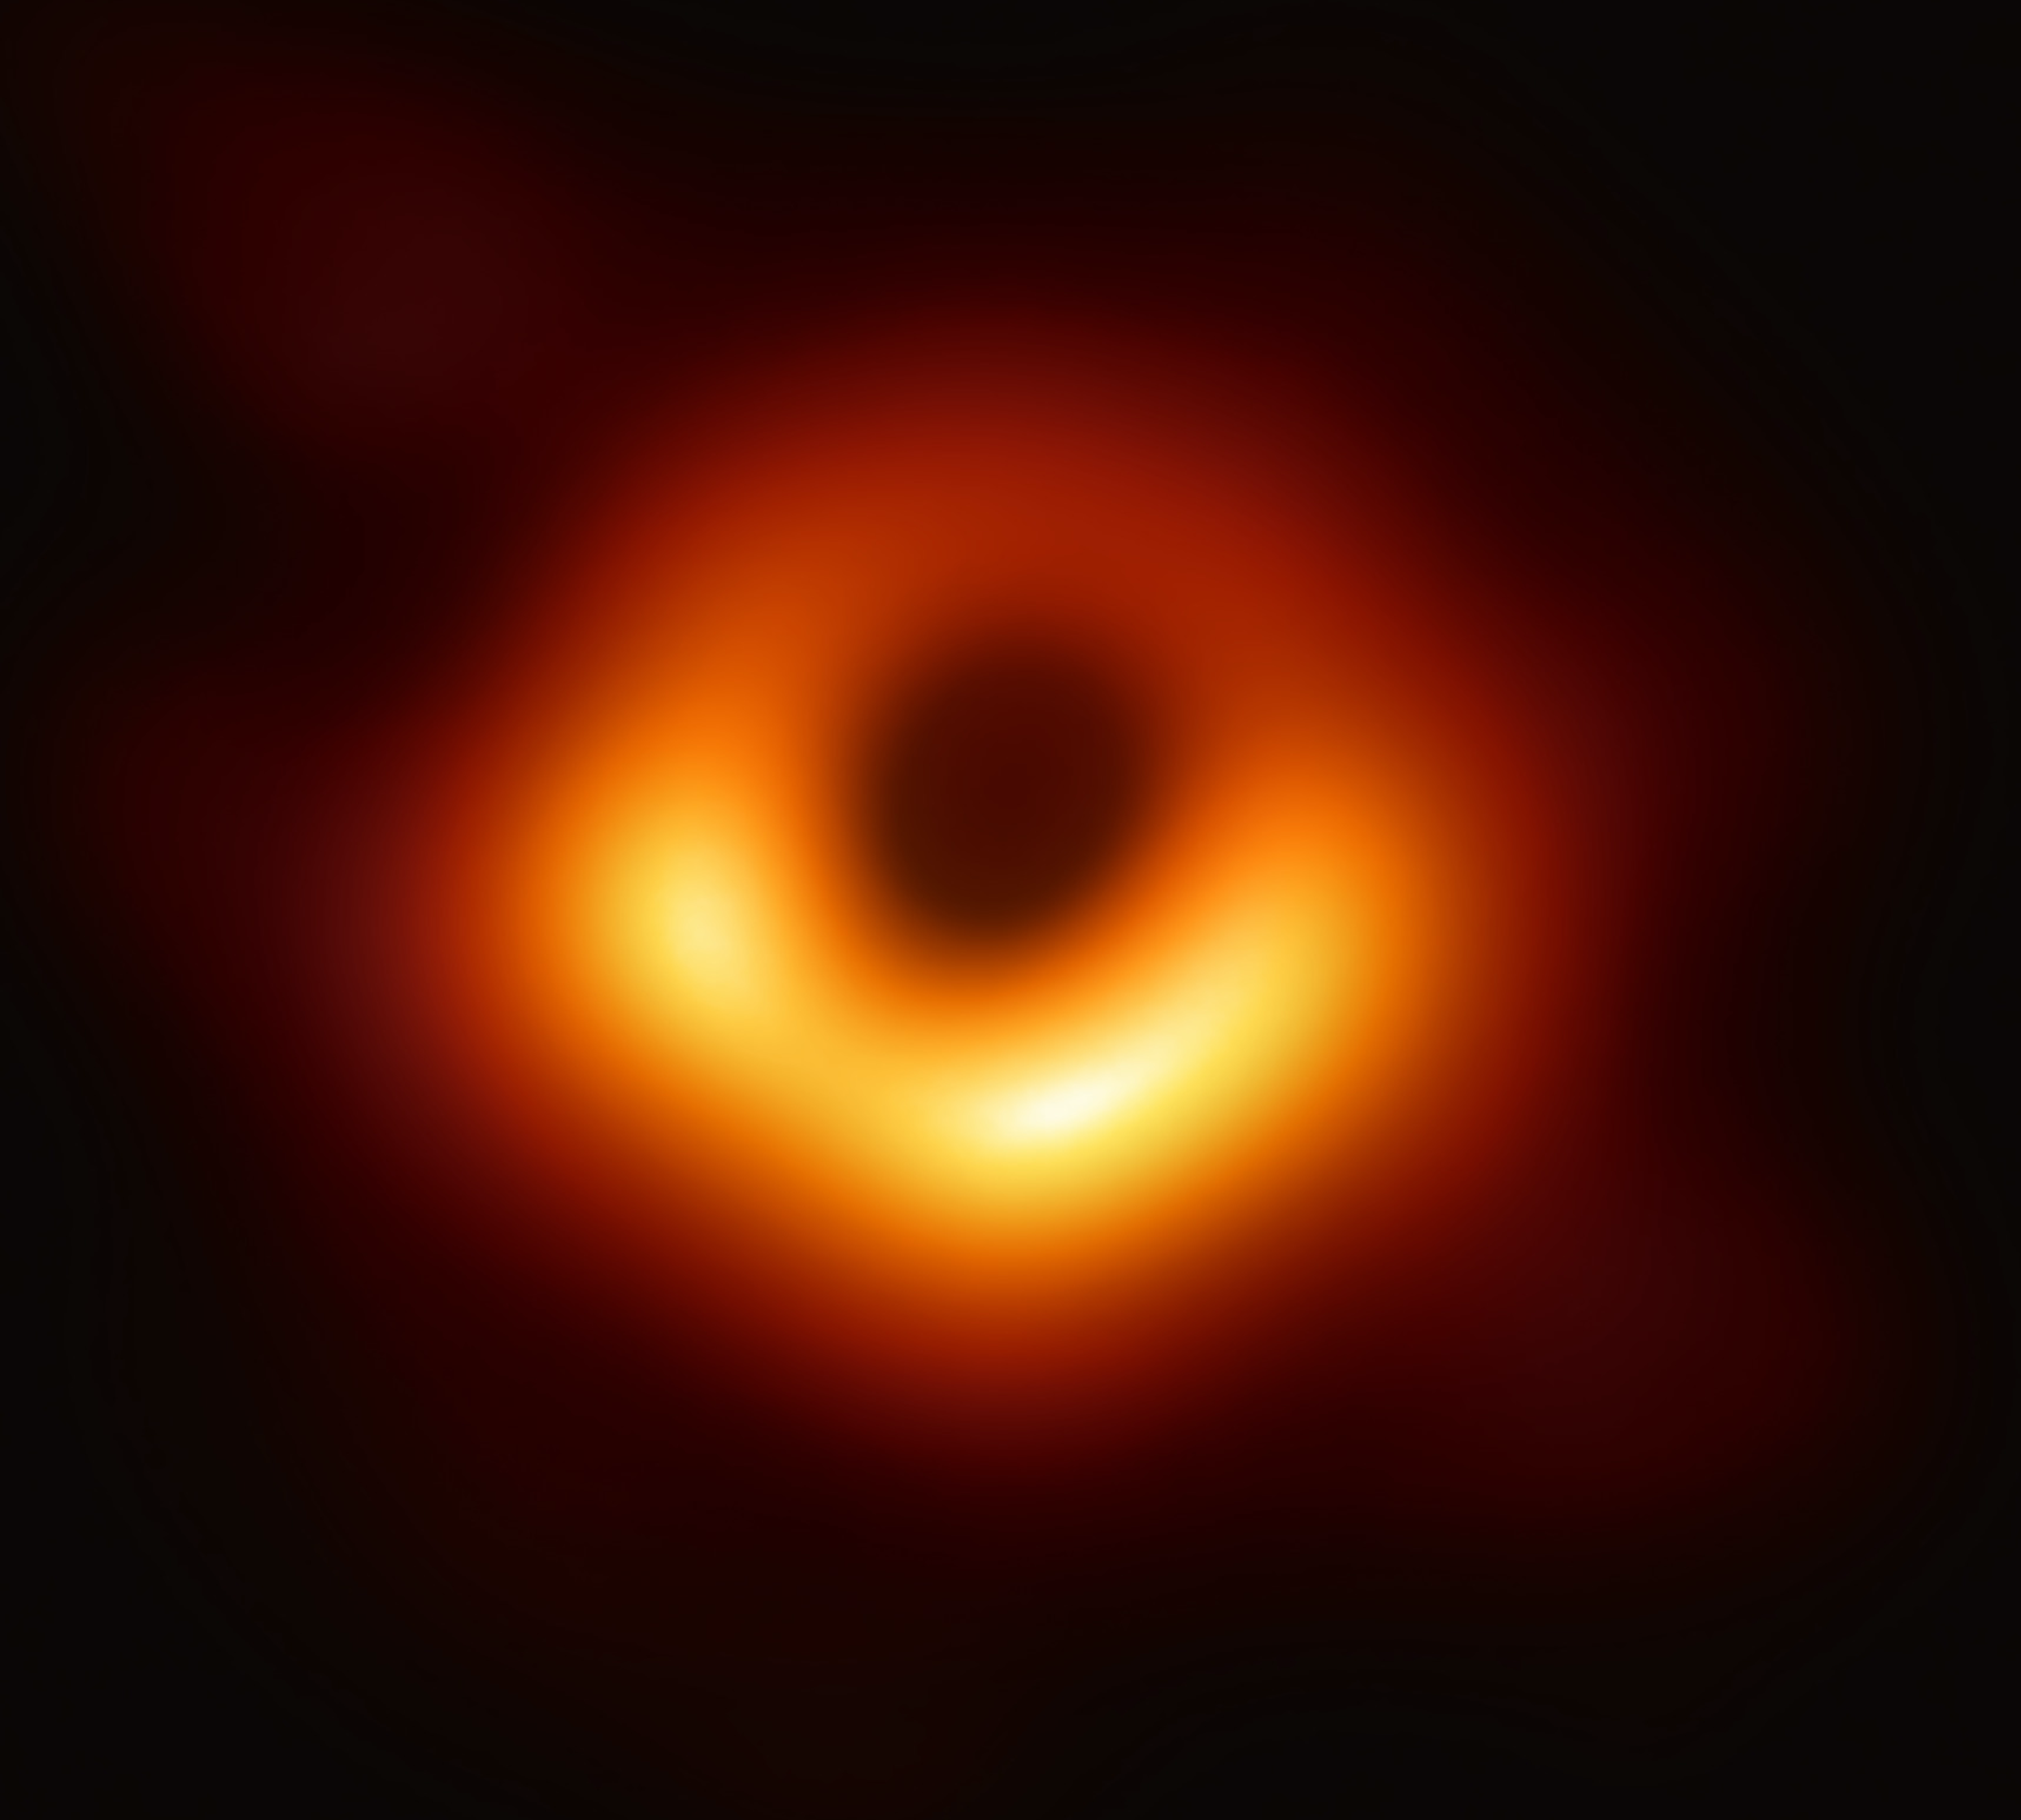
\includegraphics[width=0.88\linewidth,height=0.48\textheight,keepaspectratio]{../figs/pdf/en/fig-07-01.pdf}

% DOCX paragraph 835
\caption{\emph{Radio image, at a wavelength of 1.3 mm, of
M87\textsuperscript{*}}\index{M87*}\emph{. © The EHT Collaboration.}}\label{fig:07-01}
\end{figure}

% DOCX paragraph 837
This chapter is dedicated to the realisation of the first image of a supermassive black
hole: M87\textsuperscript{*}\index{M87*}, located at the centre of the elliptical
galaxy from where it takes its name (Messier-87, or simply M87).

% DOCX paragraph 838
Unless you have spent the last few years living on another planet or inside an isolated
cave, it is unlikely you haven't already laid eyes on the image in Figure \ref{fig:07-01}, released
by the EHT Collaboration on April 10, 2019. It is estimated that in the first 24 hours
after its release, 4.5 billion people viewed the image, which has since become almost
iconic and an inexhaustible source of comment and inspiration throughout social media.
In less than two days, the vast majority of the human population came across this image.
A record that will not be easy to beat. Even today, more than two years after that
event, sociologists and philosophers wonder why the picture of a bright half-doughnut
has attracted so much interest and become the photo of the century, worthy of a place in
the Museum of Modern Art (MoMA) in New York.

% DOCX paragraph 839
Given its popularity, it is possible many of you already know how this image was made
and why we believe it immortalises a supermassive black hole. If not, fear not: in the
following pages, I will guide you to a deeper understanding of the image, illustrating
how it was produced and how the comparison between observations and theory has brought
us to the conclusion that it is indeed a black hole.

% DOCX paragraph 840
However, before proceeding, it would be helpful to clear the ground of some speculations
made soon after the publication of the image. It has been asserted that what is
presented in Figure \ref{fig:07-01} is not a real ``photo'' but rather a map of the radio emission
by M87*\index{M87*}.

% DOCX paragraph 841
Personally, I find such considerations rather pedantic. To be clear, claims that Figure
\ref{fig:07-01} is a radio map transformed into an image are absolutely right. However, let's not
forget that every photo results from a mapping process. This is true for antique
photographic plates, where the image was reconstructed through the different light
intensities to which an emulsion of silver salts was exposed. And it is also true for
the selfies taken with smartphones, where the intensity of the electric field recorded
by a sensor placed behind the phone lens transforms into a photo of us outside the
Colosseum. It is even true for what you see right now while reading this text. The image
you perceive of the world is only a mapping of the energy distribution of
photons\index{photon} hitting the photosensitive cells located in the back of your
cornea, being transmitted through a dense network of nerves and then interpreted by the
brain.

% DOCX paragraph 842
Clearly, the point I want to make is that there is no such thing as a ``real'' photo;
everything we see is the result of the mapping of signals received and processed into an
image. And although it is undeniable that our eyes are not sensitive to the radio band,
this does not mean we cannot take a photo from this radiation. It would be like saying
that the images of our children when they were still in the womb and that many of us
still keep are not ``photos'', just because our eyes are not sensitive to the radiation
in the ultrasound band. I hope that the absurdity of this claim is evident to everyone.

% DOCX paragraph 843
To conclude, for all practical purposes, the picture in Figure \ref{fig:07-01} is the first photo of
a supermassive black hole, as produced by the EHT Collaboration. The fact that it was
made starting from a radio measurement at frequencies we humans are not sensitive to is
a completely irrelevant detail.

% DOCX paragraph 847
\section{Doing What Was Thought To Be Impossible}\label{sec:07-impossible}

% DOCX paragraph 849
Let me start this section by addressing a question that is as obvious as it is common:
``How is it possible to photograph an event horizon if, by definition, it cannot emit
light?''. The answer is simple and categorical: you can't! Photographing an object means
collecting the photons it emits, but the event horizon\index{event horizon}, by
definition, does not emit any photons, and so it is ``invisible'' for an external
observer. That said, it is possible to take a picture of what is near and around an
event horizon, especially if the horizon is surrounded by hot plasma\index{plasma}
falling onto it and emitting radiation.\textsuperscript{\hyperlink{note:07-01}{1}} That is exactly what we did
with the EHT Collaboration and is what astrophysicists are interested in.

% DOCX paragraph 850
Obviously, taking a picture of what is near a black hole does not prove the existence of
a black hole. However, suppose the observed image coincides with theoretical predictions
that can be made based on plasma\index{plasma} dynamics near an event horizon. This
then provides convincing evidence that a black hole is indeed present. Put differently,
the picture taken coincides with the image that a supermassive black hole would produce
if we got close enough.

% DOCX paragraph 851
These considerations inevitably lead to another question: ``If it is impossible to take
a picture of the event horizon, but we can image what is around it, why hasn't this been
done before?''. The answer to this question can be deduced from what we have learned
about the properties of black holes. We have seen that they are the most compact objects
in the universe, so much so that if we wanted to produce one starting from the Sun, we
would have to reduce the radius of our star to no more than 3 kilometres. Furthermore,
it is easy to understand how difficult it can be to observe a celestial object with a
radius of only 3 kilometres at astronomical distances from us, that is, well outside the
solar system.

% DOCX paragraph 852
Setting aside the fact that only a tiny part of the emission from a black hole at
astronomical distances can reach us, the most serious problem in making observations of
black holes is angular resolution\index{angular resolution}. That is, the possibility of using
a telescope (or an ensemble of telescopes) sharp enough for us to observe an object of
very small size in the sky. To give some numbers, a stellar-mass black hole very close
to us at, say, a distance of one million astronomical unit\index{AU (astronomical Unit)}s (or AU),
equal to one million times that between the Earth and the Sun, would have an angular
dimension projected on the sky of 10\textsuperscript{--10} arcseconds, or 0.0001
microarcseconds, i.e., approximately 3 × 10\textsuperscript{--14} degrees. By way of
illustration, this resolution\index{resolution|see{angular resolution}} would allow someone in Rome to
distinguish an object the size of a grain of rice in New York. There is simply no
telescope, or ensemble of telescopes capable of achieving such a angular resolution,
even using the most advanced technology. As we will see in the following pages, the best
resolution we can hope to achieve is in the order of tens of microarcseconds, and even
that would be a technological feat.

% DOCX paragraph 853
Given these considerations, it is clear that if we wanted to take a photo of a black
hole, we would need to discard stellar black holes as, obviously, they are too small to
be seen at astronomical distances. Therefore, since size grows with mass (remember the
expression of the Schwarzschild radius \ldots), we are left with supermassive black
holes. The more massive the better, so they naturally appear larger at any given
distance. Yes, distance also plays a role here because, as for any object, the more
distant the black hole is, the smaller it will appear in the sky, even if it has an
enormous mass. Hence, the ``requirements'' for the optimal candidates in this photo
contest are that they must be enormously massive and also close enough!

% DOCX paragraph 854
Once these two ``selection filters'' have been imposed among the hundreds of thousands
of supermassive black holes we presume to know in the universe, only two interesting
candidates survive. These are black holes where a projected size of about ten
microarcseconds corresponds to a physical size of about 10 Schwarzschild radii.

% DOCX paragraph 855
The two candidates left in this contest are Sagittarius
A\textsuperscript{*}\index{Sagittarius A* (Sgr A*)} (or, more simply, Sgr A\textsuperscript{*}), the
black hole at the centre of our galaxy, and M87\textsuperscript{*}\index{M87*}.
The first is interesting because, as can be guessed, it is the least distant from us;
therefore, what it lacks in mass, it compensates for with proximity (it has a mass of
``only'' a few million solar masses). On the other hand, the second candidate is more
distant from us (a thousand times more, in fact) but compensates for this with mass: it
is almost a thousand times more massive than the Sgr A* and among the most massive black
holes known to us.

% DOCX paragraph 856
Now that we have selected our ideal candidates, we had better go hunting for these black
holes ...

% DOCX paragraph 859
\section{A Telescope As Big As The Earth}\label{sec:07-telescope}

% DOCX paragraph 861
To understand how the image in Figure \ref{fig:07-01} was made, we first need to discuss the
technical and technological aspects of the observations. For this reason, and in the
spirit of inducing an appreciation of how mathematics is at the origin of all physical
understanding, let me show you the following conceptual equation, which is easy to
understand and very general:

% DOCX paragraph 863
\begin{equation}\label{eq:07-01}
\begin{pmatrix}\text{angular resolution of} \\ \text{astronomical image}\end{pmatrix}
=\left(\frac{\text{wavelength of observations}}{\text{telescope size}}\right)
\end{equation}

% DOCX paragraph 864

% DOCX paragraph 866
Equation \eqref{eq:07-01} tells us that if we want to achieve a very small angular
resolution\index{angular resolution} (so we can distinguish tiny details and study objects
whose projected size on the sky is very small), we must ensure the ratio between the
wavelength at which we make the observations, and the size of the telescope is as small
as possible.

% DOCX paragraph 867
You may think the simplest way to reduce this ratio would be to make observations at the
shortest possible wavelengths, namely, those in the X-ray\index{X-ray!radiation} or even
gamma-ray\index{gamma-ray|see{astronomy}} \index{radiation!gamma-ray}band. But unfortunately, this is not an
option; the simple reason is that we do not receive, and cannot receive,
X-ray\index{X-ray!radiation} or gamma-ray radiation from a supermassive black hole. To
understand why this is the case, we need to appreciate the difference between the
radiation emitted and the radiation that reaches our telescopes.

% DOCX paragraph 868
A supermassive black hole accreting matter from its surroundings will emit
electromagnetic radiation\index{radiation!electromagnetic} in a very wide spectrum\index{spectrum!electromagnetic}.
Also, as we have seen for Cyg-X1, this radiation is extremely strong at wavelengths in
the X- and gamma-ray bands. Such emissions are generated very close to the event horizon
--- precisely the region we are most interested in regarding our observations. However,
the emission of radiation is a necessary but not sufficient condition for a successful
astronomical observation, as we also need the radiation to reach our telescopes.
Unfortunately, this is not the case with the X- and gamma-ray (and optical) bands. The
reason is that there is quite a bit of matter between us and the source, either in the
form of accreting plasma\index{plasma!accreting} under extreme conditions of temperature and
energy or in the form of simple interstellar dust. In both cases, this matter is very
effective in absorbing the radiation before it can reach us. As a result, although the
accreting material around a supermassive black hole does indeed emit light over a very
broad spectrum\index{spectrum!electromagnetic}, much of it is absorbed or scattered, never reaching
our telescopes.

% DOCX paragraph 869
To help understand the meaning of absorption and scattering, let me offer an analogy.
Take the sky on a cloudy day: if the cloud cover is not particularly dense and there is
only a thin veil of clouds, we will still be able to see the silhouette of the Sun,
which will appear as a brighter spot in the sky. However, if the cloud cover is very
dense, then our favourite star will not be visible because the clouds will absorb the
radiation it emits, so it will not reach us, or at least not directly. But, in reality,
sunlight on a cloudy day does reach us (indeed, a cloudy day is not as dark as night).
This is because the photons emitted by the Sun are scattered countless times by the
water vapour\index{water vapour} molecules in the clouds, giving rise to the typical
shadowless brightness of a gloomy day.

% DOCX paragraph 870
Let's go back now to Equation \eqref{eq:07-01}. To decide which wavelength to use for our
observations and thus establish which resolution we can hope to obtain, we have to
resort not to the smallest wavelength emitted but to the smallest that can be received
on Earth. Omitting details concerning a comprehensive model of the radiation emitted
near a black hole, the optimal wavelength for imaging a supermassive black hole turns
out to be in the \emph{radio band} and is of the order of 1.3 millimetres, thus
corresponding to a frequency of about 230 GHz. This wavelength is a million times longer
than that of X-ray\index{X-ray!radiation} radiation (which is around one nanometer), but it
has the advantage that the plasma around the black hole is almost transparent to this
radiation, which can therefore reach us without being absorbed or scattered along its
path.

% DOCX paragraph 871
Having established that we need to collect radiation in the radio band, we must now
tackle a much more difficult problem: we need to collect it! In particular, we have to
find a radio-telescope large enough to allow us to obtain a resolution of a few tens of
arc microseconds. Fortunately, radio-telescopes of considerable size can be built, as
they are basically just steel structures similar to oversized satellite TV dishes. While
most radio-telescopes have diameters of between 20 and 50 metres, there are two that are
decidedly larger: the radio-telescope at the Arecibo\index{radio-telescope!Arecibo} Observatory in
Puerto Rico and the FAST telescope\index{radio-telescope!FAST} in China, whose diameter is 500
metres across. Unfortunately, however, not even such an enormous radio-telescope would
be able to obtain the resolution we need, failing by at least five orders of magnitude!
In fact, if you were to use Equation \eqref{eq:07-01} to determine the size of radio-telescope
required to reach a resolution of about ten microarcseconds at a wavelength of one
millimetre, you would find that you need a telescope of about 10,000 kilometres in
diameter! In other words, the telescope would have to be as large as the entire planet!

% DOCX paragraph 872
While this may appear to be an impossible feat, human ingenuity has allowed us to use
the whole planet as a telescope by developing, in the 1980s, a radio-astronomical
technique now widely used: the Very Long Baseline Interferometry\index{VLBI (Very Long Baseline Interferometry)}, or
VLBI.

% DOCX paragraph 878
\section{A Most Amazing Technique}\label{sec:07-vlbi}

% DOCX paragraph 880
We can avoid going into the details of the VLBI technique here, as some are rather
sophisticated. Instead, it is sufficient to recall that interferometry exploits the
property of ``linear superposition'' of wave phenomena, whether they be
electromagnetic\index{waves!electromagnetic}, sound\index{waves!soumd}, or seismic
waves\index{waves!seismic}. This property allows waves to be combined in what is known as
interference\index{interference}\index{waves!interference}. This interference can then be
constructive\index{interference!constructive} when the amplitude of the waves adds up or
destructive\index{interference!destructive} in the opposite case. The VLBI technique is designed to
exploit the interference between the signals received by two radio-telescopes placed
thousands of kilometres away from each other, such as the
radio-telescope\index{radio-telescope!Pico Veleta} at Pico Veleta in Spain and the ALMA
telescope\index{radio-telescope!ALMA (Atacama Large Millimiter Array)} in Chile. In this way, it is as if a single \emph{virtual}
radio-telescope has been constructed with a diameter equal to the distance between the
two \emph{real} radio-telescopes.

% DOCX paragraph 881
The VLBI technique is truly amazing, to the point of appearing almost too good to be
true, and thus raising the doubt: ``Where's the catch?''. Of course, in reality, there
is no catch, but it should be recognised that the VLBI technique comes with precise
constraints, some of which are rather tight.

% DOCX paragraph 882
The first such constraint is to guarantee that the two radio-telescopes observe the same
object at the same instant in time. The reason behind this requirement is quite obvious.
Without perfect tuning between the two telescopes, there would be no certainty that they
measure the same wavefront of electromagnetic radiation\index{radiation!electromagnetic}.
Consequently, this would invalidate the whole interferometric process, and the
observations would not lead to an image.

% DOCX paragraph 883
Let me remind you that light propagates as a wave and that the wavefronts of the light
emitted by sources at astronomical distances reach the Earth as plane and parallel
fronts. To ensure that two different telescopes record the same wavefront, the reading
of the electric field measured by the radio receiver (even your home radio records a
time-varying electric field) must be combined with the reading of the moment of arrival
of the wavefront. For this purpose, each of the two telescopes must be equipped with an
extremely precise atomic\index{atomic!clock} clock to mark the time of arrival of the
electrical signal.

% DOCX paragraph 884
The second constraint of the VLBI technique is that the image cannot be produced in
real-time but only after correlating the signals of two (or more) telescopes. For this
reason, each observation, which alone produces enormous amounts of data (of the order of
hundreds of terabytes), must be recorded and sent to a special supercomputing centre,
where different data streams combine to create the interferometry between the two
telescopes. Further complicating matters, it is almost impossible to transfer data via
the internet as radio-telescopes are located where visibility is optimal but at sites
that are often isolated and difficult to reach (one of the EHT telescopes is at the
South Pole!). Notably, they are typically built in extremely arid areas --- water
vapour\index{water vapour} is the greatest enemy of radio observations. For this reason,
once recorded on physical media, the data must be transferred (usually using students as
couriers) to the supercomputing centre in charge of data combination.

% DOCX paragraph 885
The details we have discussed so far should have provided you with an initial idea of
the technological complications associated with the VLBI technique and revealed, at
least in part, how complex it is to employ this advanced technique in practice. Yet,
with its observations, the EHT has further raised the bar of this technological
sophistication in at least two ways. The first is through the number of radio-telescopes
used. The principle of the operation, previously described, between two telescopes can
extend to an entire network of instruments, each connected individually to any other
telescope in the network. Doing this gains two important advantages: to increase the
image quality and to extend the observation times. When only two radio-telescopes are
used, the resulting interferometric image is approximate and contains only the main
basic features. Therefore, it is advantageous to use as many radio-telescopes as
possible to improve this and obtain additional detail in the image. Besides obtaining
more information and, therefore, detail in the image, having more radio-telescopes
available also means that the source can be ``followed'' over longer timescales. This is
because when the source disappears below the horizon of one telescope due to the Earth's
rotation, it will still be detectable by others for which the source has just appeared
in the sky. For example, on any given day, the radio-telescope at Pico Veleta, in Spain,
will be the first to record a source such as M87*\index{M87*}, while the JCMT
telescope\index{radio-telescope!JCMT (James Clerk Maxwell)} in Hawaii will be the last. Using eight different
radio-telescopes distributed across the planet, the EHT Collaboration has achieved
unprecedented operational continuity and conducted observations over a time frame of
between eight and ten hours a day --- five times longer than with just two
radio-telescopes. In turn, this prolonged observation time has considerably improved the
quality of the reconstructed images produced by the EHT Collaboration.

% DOCX paragraph 886
It should be emphasised that the simultaneous management of eight radio-telescopes
distributed in remote areas of different continents is by no means a trivial operation.
Especially since the EHT does not ``own'' or manage these telescopes. Instead, the EHT
obtained access to the telescopes after winning a highly competitive public application
process that provides the availability of the telescopes to carry out the observations.
Having obtained a common time frame for the radio-telescopes in April 2017, EHT
scientists were sent to the various sites to undertake observations and \ldots{} to wish
for favourable weather conditions. While radio-telescopes can operate day and night, the
weather does play a critical role because, as mentioned, water vapour\index{water vapour}
considerably reduces the quality of the signal received. Although seemingly paradoxical,
in 2017, EHT scientists were trying to collect light coming from 65 million light years
away (light that had taken 65 million years to reach us), and they had to hope that a
cloud just a few kilometres above the ground would not absorb the radiation a fraction
of a second before it reached the telescope!

% DOCX paragraph 887
The second reason why the EHT Collaboration has taken the VLBI technique to the
forefront of its capabilities is its use of radio-telescopes observing at the maximum
frequency of current technology, namely 230 GHz. In turn, this has guaranteed the best
possible resolution to date, namely, about ten microarcseconds (recall Equation \eqref{eq:07-01}).

% DOCX paragraph 888
To help you appreciate the astounding ``zoom'' capability achieved by the EHT resolution
in M87*\index{M87*}, Figure \ref{fig:07-02} provides a composition of radio images showing
how the M87\index{M87!images} galaxy appears at different frequencies. The figure
reports the radio frequency employed, the angular resolution\index{angular resolution}
obtained, and the corresponding length-scale for each image.

% DOCX paragraph 889
As you can see, the radio-telescopes\index{radio-telescope!VLA (Very Large Array)} at the Very Large Array (VLA) in
New Mexico operate at a frequency of 1.5 GHz and produce an image with an angular
resolution\index{angular resolution} of 10 arcseconds, corresponding to a scale of three
thousand light years. In this image, we can note the presence of two jets: one, clearly
visible, which moves to the right, the other directed to the left and identifiable only
at the end of its trajectory, when it collides with the interstellar medium (i.e., the
mix of dust and rarefied gas found among stars). Instead, by increasing the observation
frequency to 43 GHz, the radio-telescopes of the Very Long Baseline Array (VLBA)
\index{radio-telescope!VLBA (Very Large Baseline Array)} in the USA can reconstruct an image with a resolution a thousand
times higher (namely, 0.01 arcseconds). This allows us to better visualise the interior
of the jet over a length-scale of three light years. Similarly, the Global 3-mm VLBI
Array (GMVA) \index{radio-telescope!GMVA (Global 3-mm VLBI Array)} telescope can operate at a frequency twice as large, 86
GHz, with telescopes that are further apart, thus increasing the resolution by a factor
of one hundred, namely, 0.0001 arcseconds, which corresponds to a length-scale of a
fraction of a light year. Finally, the enormous technological effort made by the EHT,
whose observations have been carried out at 230 GHz, have yielded an image with a
resolution of the order of ten microarcseconds, corresponding to a length-scale of only
three light hours.

% DOCX paragraph 890
\begin{figure}[htbp]
\centering
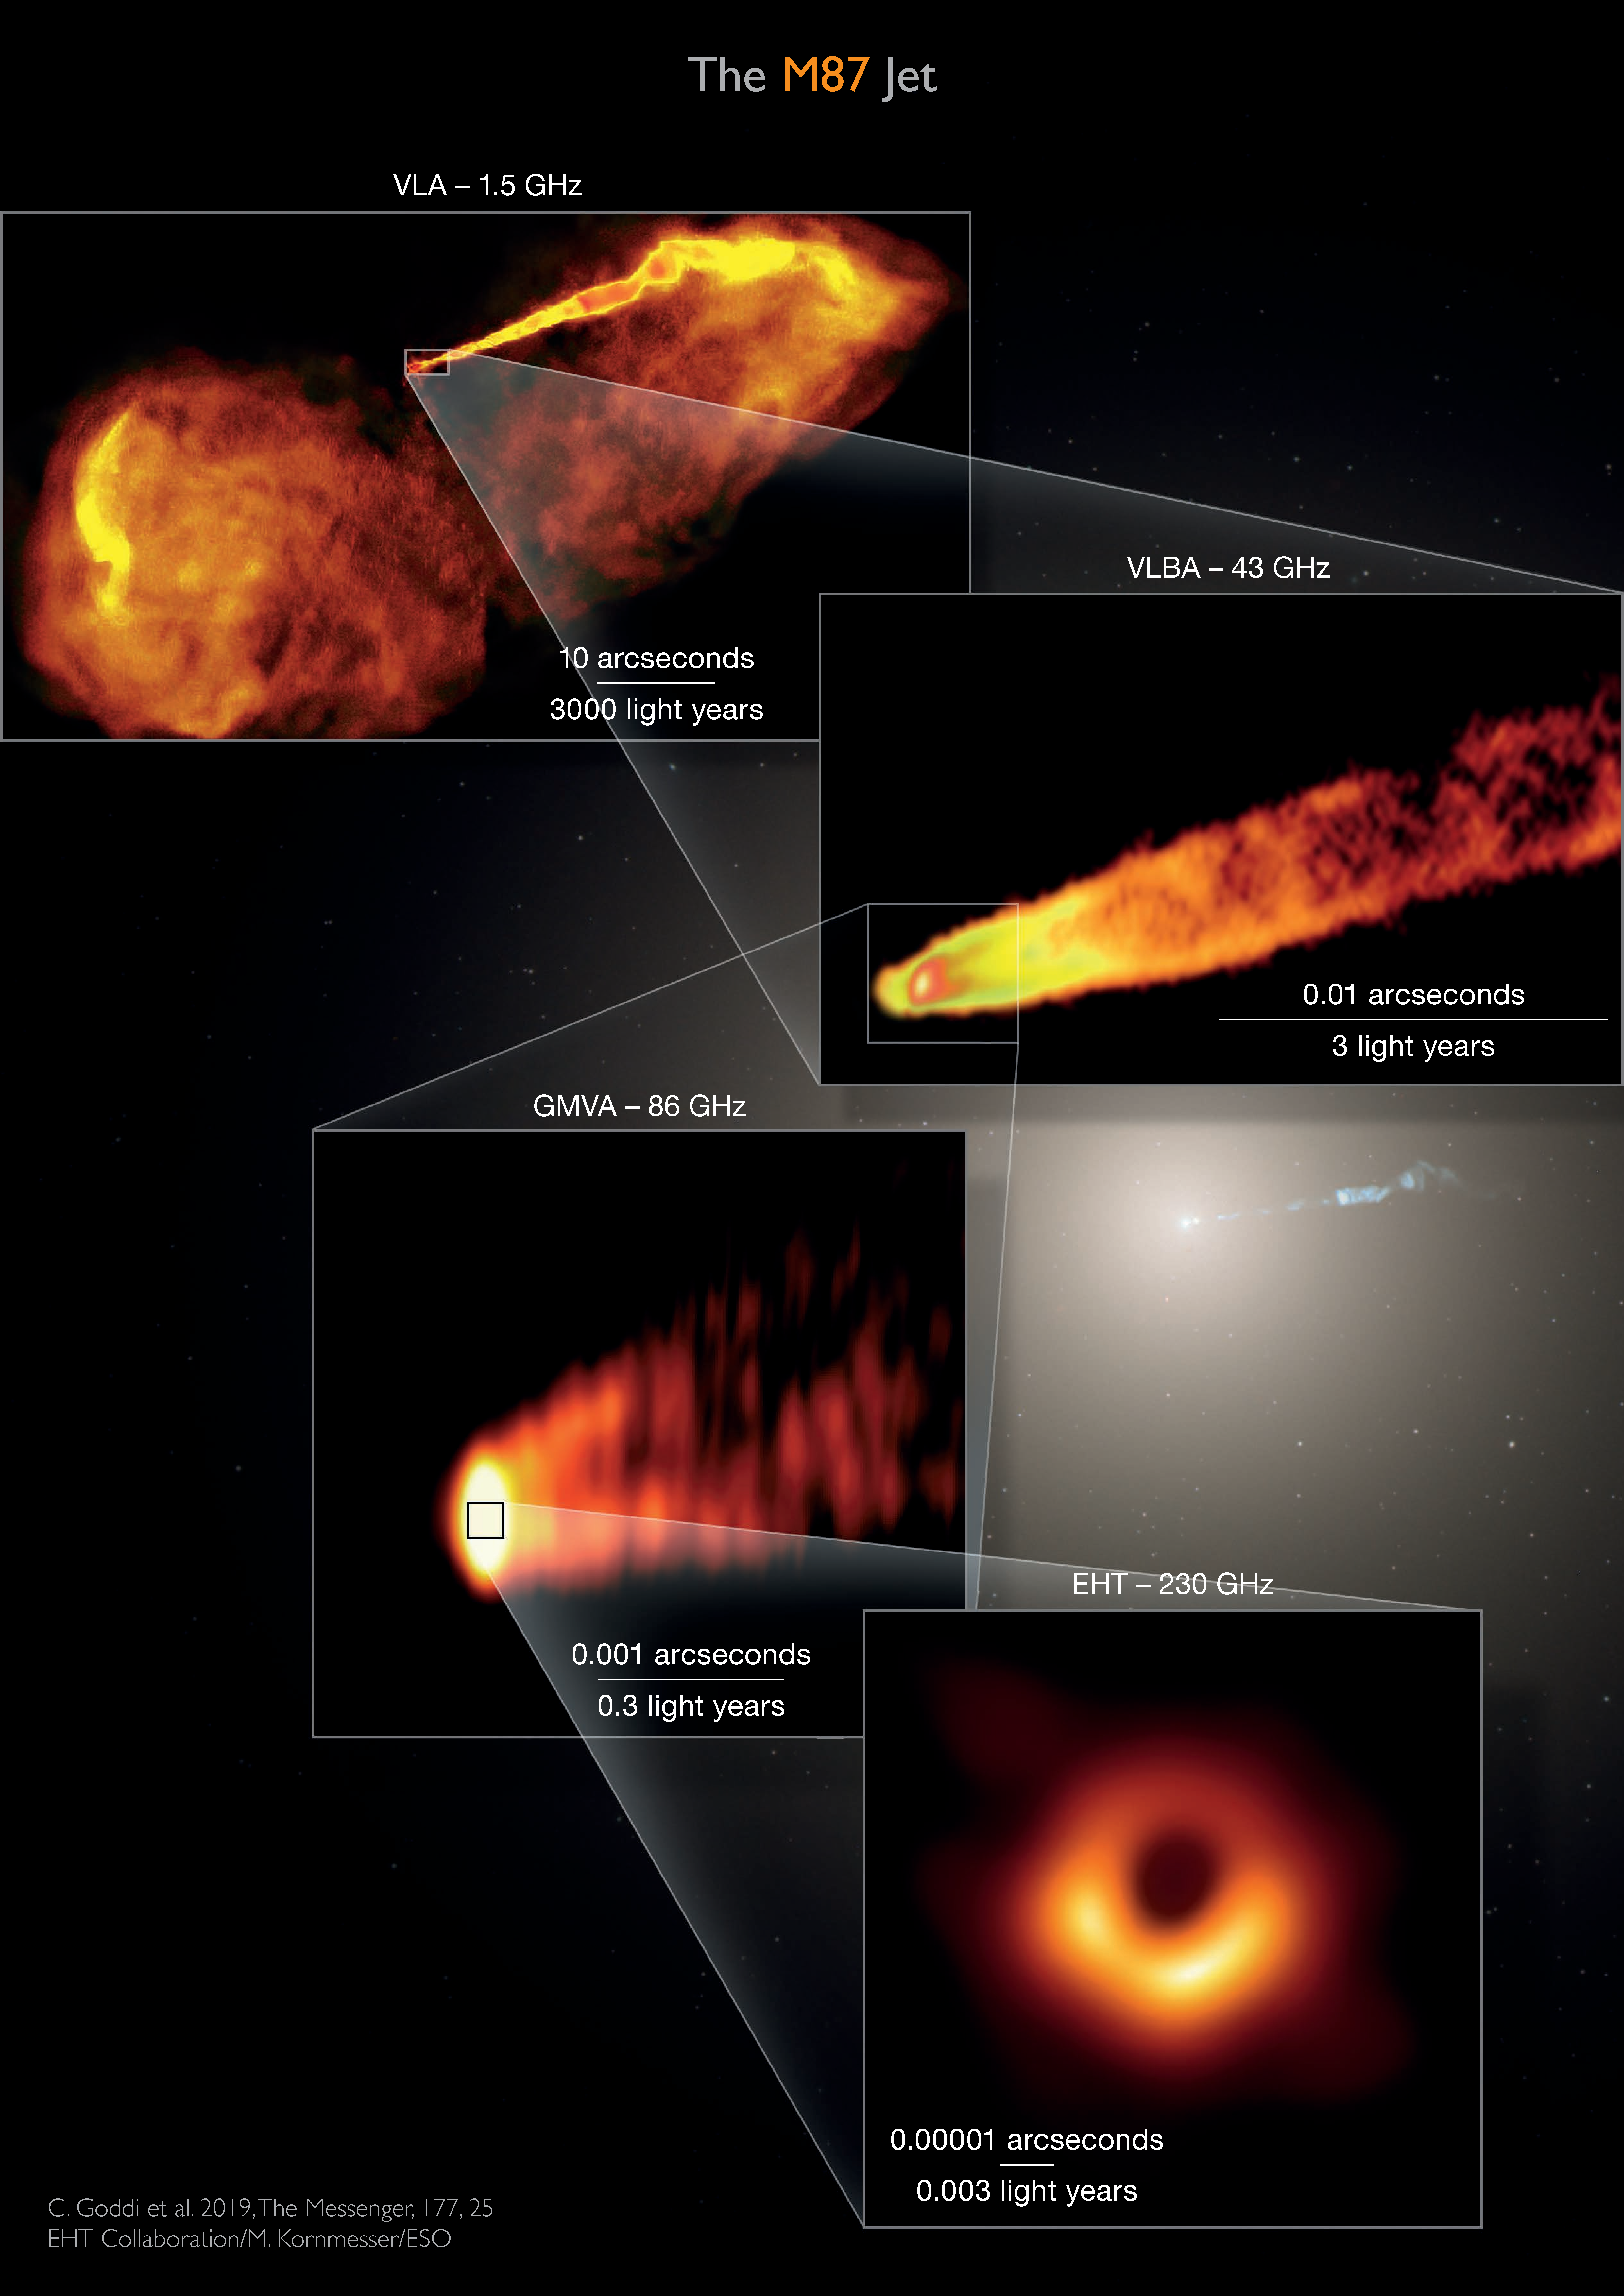
\includegraphics[width=0.96\linewidth,height=0.74\textheight,keepaspectratio]{../figs/pdf/en/fig-07-02.pdf}

% DOCX paragraph 892
\caption{\emph{Image composition of M87 at different radio frequencies, and therefore at
different angular resolutions. © The EHT Collaboration/ESO/M. Kornmesser/C. Goddi/LR.}}\label{fig:07-02}
\end{figure}

% DOCX paragraph 894
In the background of Figure \ref{fig:07-02}, there is an image of the whole galaxy M87 taken in the
optical band. It appears as an object with a diffused brightness and a bright core, from
which the right moving jet seems to emerge as a collimated plume of smoke (the left
moving jet is absorbed almost entirely at these wavelengths).

% DOCX paragraph 895
At this point, I think it is clear why an image like the one produced by the EHT is the
first of its kind. In order to produce and interpret the image, it was necessary to
bring together a considerable number of scientists from every stage of the process, all
the way from observations to theory. As in other scientific efforts of this type,
success inevitably depends on the availability of significant economic resources to
finance the work of so many scientists. It is not without a hint of pride that the
European scientific community has provided an important, if not essential, contribution
in this regard. In fact, it is thanks to the substantial funds assigned by the European
Research Council\index{ERC (European Research Council)} (or ERC) in 2013 to myself and my colleagues, Heino
Falcke (University of Nijmegen in the Netherlands) and Michael Kramer (Max-Planck
Institute in Bonn, Germany), that it was possible for the EHT (whose formal foundation
dates back to 2009) to ``take off'' in 2014 as an effective collaboration and to carry
out the much needed research. The fourteen million euros, obtained via our ERC Synergy
Grant, BlackHoleCam\index{BlackHoleCam}\textsuperscript{\hyperlink{note:07-02}{2}} (the largest grant made by the
European Research Council to Astronomy), made it possible to set up a team of leading
European researchers and has been a catalyst for the granting of additional funds for
American and Asian colleagues. Only in this way, and after reaching the necessary
``critical mass'', was it possible to transform the idea of taking a picture of a
supermassive black hole into a reality.

% DOCX paragraph 896
I will end this section with an intriguing comment on the role luck plays in human
activities, including those that we, as scientists, strive to remove as much as possible
from the will of fate. As discussed above, the EHT has achieved the highest angular
resolution\index{angular resolution} ever obtained in radio astronomy for a supermassive black
hole. Yet this resolution was barely enough to produce with confidence an image of
M87*\index{M87*}, whose projected image on the sky is a few tens of
microarcseconds. This knowledge, however, is available to us only now that we have an
estimate for the mass of M87*. Before 2017, the mass of M87* was still uncertain and the
various estimates differed by a factor of two. Hence, had the mass of M87* been only a
factor of two smaller (as one of the estimates claimed), its image in the sky would have
been correspondingly smaller by a factor of two and the EHT resolution insufficient, no
matter how revolutionary. Because we didn't know all of this back then, the EHT
observations in 2017 were, in part, an educated guess. Nevertheless, the lesson is
always the same: ``fortuna iuvat audaces'' (fortune favours the bold). And, in the EHT
Collaboration we were as bold as we were lucky ...

% DOCX paragraph 899
\section{All A Matter Of Trajectories}\label{sec:07-trajectories}

% DOCX paragraph 901
Now that we have a better idea of the technology involved in making VLBI observations,
we can finally turn our attention to what happens to light rays in the vicinity of a
black hole. Knowing the possible trajectories light can travel on is most important in
understanding why the image of M87*\index{M87*} must necessarily be as shown in
Figure \ref{fig:07-01}.

% DOCX paragraph 902
We have already discussed in Chapter 3 that nothing can move in a straight line within a
curved spacetime, not even light rays (photons) \index{photon!orbits} insomuch that they
can give rise to gravitational lensing\index{gravitational!lensing} phenomena. Since spacetime
reaches its maximum curvature precisely near black holes, it is natural to expect that
photons will take very curved trajectories in these regions. And that's exactly right!

% DOCX paragraph 903
We can see this, for example, in Figure \ref{fig:07-03}, which shows the trajectories travelled by
some photons near a Schwarzschild black hole\index{black hole!Schwarzchild}, therefore a nonrotating
black hole. When seen for the first time, I know that this figure can be intimidating or
even confusing, but let's go through it patiently together and try to understand all of
the information.

% DOCX paragraph 905
\begin{figure}[htbp]
\centering
non-rotating\par\medskip

% DOCX paragraph 906
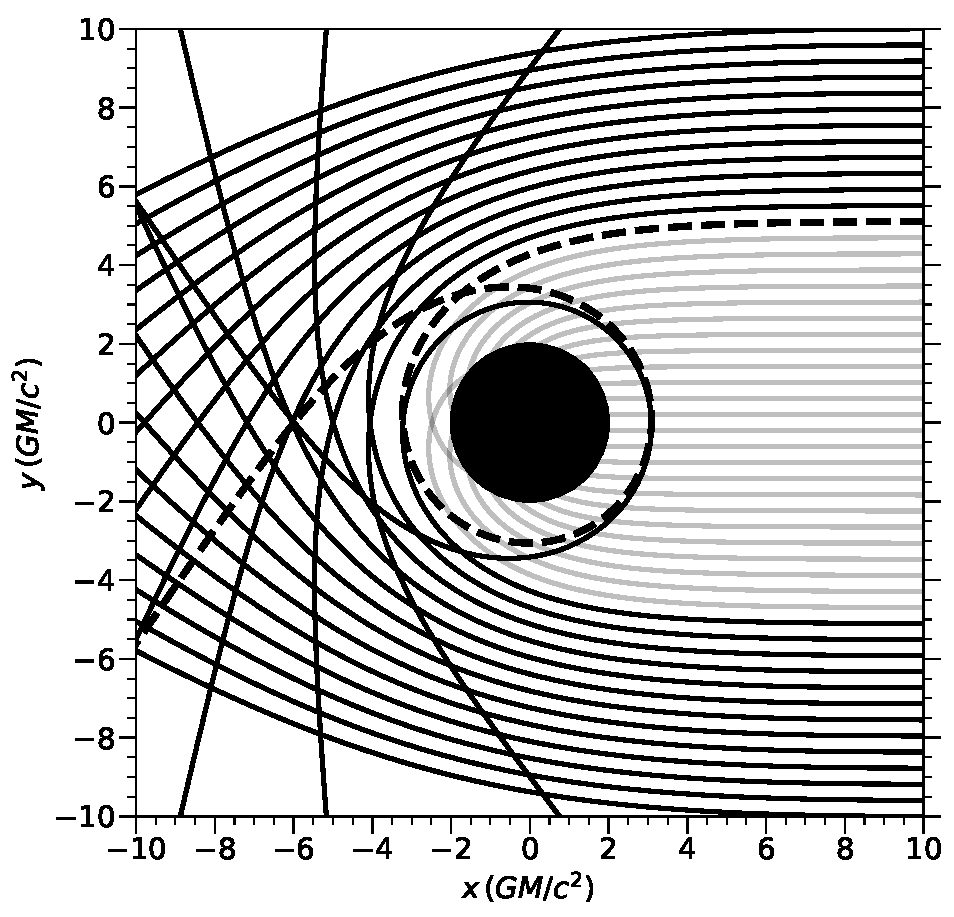
\includegraphics[width=0.88\linewidth,height=0.48\textheight,keepaspectratio]{../figs/pdf/en/fig-07-03.pdf}

% DOCX paragraph 908
\caption{\emph{Photon orbits}\index{orbit!photon} \emph{on the equatorial plane, oriented
from right to left, of a nonrotating black hole. © C. Fromm/LR.}}\label{fig:07-03}
\end{figure}

% DOCX paragraph 910
To begin with, Figure \ref{fig:07-03} indicates the motion of photons\index{orbit!photon} on an
equatorial plane, with the dark circle in the centre representing the event
horizon\index{event horizon} of a black hole as seen from above. Furthermore, the
trajectories refer to light rays emitted, all starting from the right of the figure, at
\emph{x=10 (GM/c\textsuperscript{2})}, so you can follow any of these trajectories from
their origin, for example, the top one would be at \emph{x=10 (GM/c\textsuperscript{2})}
and \emph{y=10 (GM/c\textsuperscript{2})}, and proceed from right to left.

% DOCX paragraph 911
It is fairly obvious that some trajectories are deflected but do not end up in the black
hole (indicated with solid black lines), while others are captured by the black hole and
end up inside the event horizon (indicated with solid grey lines). Immediately apparent
is that the trajectories farthest from the black hole are deflected only slightly, but
also that, as they get closer to the black hole (or, to be more precise, as the impact
parameter\textsuperscript{\hyperlink{note:07-03}{3}} decreases), the deflection becomes larger and larger, until
it is greater than 90 degrees. Note that, among the trajectories captured by the black
hole, some enter ``directly'' into the event horizon without undergoing a significant
deflection, while others are captured after passing near the black hole. Finally, a
dashed black line shows an example of the bizarre trajectories that can develop near a
black hole. In this case, the photon starts from \emph{x=10 (GM/c\textsuperscript{2})}
and \emph{y≃5.2 (GM/c\textsuperscript{2})}, it approaches the black hole, completes an
entire revolution around it, and moves away at \emph{x=-10 (GM/c\textsuperscript{2})}
and \emph{y≃--5.5 (GM/c\textsuperscript{2})}. Clearly, this is a ``strange'' orbit, to
say the least, but soon we will see there are even more bizarre ones.

% DOCX paragraph 912
Looking at Figure \ref{fig:07-03}, we can imagine a limit between the black trajectories (deflected
but not captured) and the grey trajectories (deflected and captured). This limit is
represented by the unstable circular orbit\index{orbit!unstable circular (photon)} of photons, or
\emph{``light ring''}, and, in the case of a Schwarzschild black
hole\index{black hole!Schwarzchild}, is located at a precise radius\textsuperscript{\hyperlink{note:07-04}{4}}:
\emph{r\textsubscript{po}=3 (GM/c\textsuperscript{2})}. Therefore, Figure \ref{fig:07-03} shows us
that a very special trajectory for a light ray around a nonrotating black hole must
exist. Thus, if we placed, with great precision, a beam of light on this orbit, it could
ideally remain on the same radius, that is, the photon ring\index{photon!ring (light)}, forever.
However, this happens to be an ``\emph{unstable''} orbit\index{orbit!unstable circular (photon)}, and a
photon moving along it would feel very much as we would if we were walking on top of a
razor-sharp crest of a mountain chain with very steep sides; the slightest disturbance
would make us fall to one side. Similarly, the slightest perturbation would make the
photon leave the light ring and either fall into the black hole or move away to
infinity.

% DOCX paragraph 913
To provide a concrete picture of what happens to photons near a black hole, I usually
use a mechanical analogy based on a bow and some arrows. Imagine a target with
extraordinary properties: just like a standard target, if an arrow meets it directly
along its trajectory, it can be hit. At the same time, because it is a special target,
it can also be hit if an arrow flies sufficiently close because the target forces the
arrow to turn around (once or multiple times) until it hits it. I admit I have often
wished that such a target really did exist as it would have greatly improved my
performance as an archer~... However, this is pretty much what happens to all the
photons grazing the black hole within the light ring: they do not need to hit the event
horizon\index{event horizon} directly because, sooner or later, they will fall into it
anyway. Soon we will see how the limiting trajectory given by the light ring plays a
decisive role in the observations of a black hole.

% DOCX paragraph 916
\section{The Vortical Motion Near A Rotating Black Hole}\label{sec:07-rotation}

% DOCX paragraph 918
The behaviour of the light rays shown in Figure \ref{fig:07-03} can also be extended to rotating
(Kerr) black holes, which represent the vast majority of the black holes in the
universe. However, before discussing the motion of light near such black holes, it is
necessary to introduce an important feature of rotating black holes that we have not
discussed yet. We have seen that black holes generate extreme curvature in the spacetime
surrounding them. For the same reason, if they are rotating, it is natural to expect
that their motion will somehow also induce a ``rotation'' of the spacetime. In other
words, it is plausible to expect that a rotating black hole will generate a kind of
vortex of curvature in spacetime around itself, forcing any object that is close by to
rotate with it.

% DOCX paragraph 919
To understand what is going on, let's imagine taking a test particle\index{test particle}
at a great distance from a rotating black hole and that this particle has no angular
momentum (i.e., the particle will not be rotating with respect to a local reference
system). If we drop the particle, it will naturally fall towards the black hole,
following a trajectory that is, at least initially, a purely radial one. However,
something bizarre happens as the particle approaches the rotating black hole. To a
distant observer, its trajectory no longer appears to be purely radial, but it also
acquires a spiral motion, as if it were rotating in the same direction as the black
hole. Not surprisingly, if we were to repeat exactly the same experiment with a
nonrotating black hole, we would find very different behaviour: the test particle would
continue moving on a radial trajectory until it reached the event horizon. This
phenomenon, the induced rotation of a test particle, is technically referred to as the
``dragging of inertial frames'' and embodies a characteristic property of rotating black
holes.

% DOCX paragraph 920
The dragging into rotation of the surrounding spacetime is not unique to black holes but
also occurs with neutron stars and planets (this phenomenon has even been recorded for
the Earth!). However, the strength of this behaviour again becomes extreme in the case
of black holes. A rotating black hole has a very special surface located outside the
event horizon\index{event horizon}, named the
``\emph{ergosphere}\index{black hole!ergosphere}''\index{ergosphere|see{black hole}}, or ``\emph{static
limit}\index{static limit}''. The properties of this surface are such that any object,
with or without mass, can rotate in the opposite direction to the black hole (i.e., it
can counter-rotate) as long as it is outside the ergosphere\index{orbit!counter-rotating}. However,
once it has crossed the ergosphere, it will no longer resist the rotation of the black
hole and will therefore be forced to rotate in the same direction (i.e., to corotate).

% DOCX paragraph 921
To better understand the role of the ergosphere, we could use an analogy from the
previous chapter for a nonrotating black hole and a lake with a hole at the bottom. If
you remember, we imagined a circular waterfall where the water fell along radial
trajectories. Instead, we can now imagine that the hole rotates or, equivalently, that
the falling water has a certain angular momentum. This would create a vortex near the
waterfall where, at large distances from the hole, the current would remain essentially
radial and become more and more vortical the closer it got to the hole. If we were on a
boat and simply let the current carry us towards the hole, we would naturally rotate
together with the rest of the water. However, at sufficiently large distances, we could
use the powerful engines on our boat to resist the current and counter-rotate in
relation to the hole, although doing this would become increasingly difficult as we
approached the waterfall. In particular, there would be a critical point beyond which,
regardless of the power of our engines, we would not be able to rotate against the
current and would instead be forced to corotate. This critical point is the mechanical
equivalent of the ergosphere in a rotating black hole.

% DOCX paragraph 922
It is essential to underline that when inside the ergosphere, we will no longer be able
to oppose the sense of rotation imparted by the black hole, but we will still be outside
the event horizon. So, in principle, we can still get out of the ergosphere, for
example, by following a partially radial motion and, therefore, moving to large
distances from the black hole. This is possible because the outer limit edge of the
ergosphere\index{black hole!ergosphere} does not behave like an event horizon (indeed, it is at a
radius larger than the event horizon), thus allowing both ingoing and outgoing motion.

% DOCX paragraph 923
Figure \ref{fig:07-04} illustrates this in a very schematic manner, showing the vortical motion of
the spacetime near a black hole and the position of the outer edge of the ergosphere,
which is clearly located at a radius larger than that of the event
horizon\index{event horizon}. Outside the ergosphere, it is possible to counter-rotate.
However, it is impossible to counter-rotate in the region between the ergosphere and the
event horizon, but it is possible to move out to large distances. Inside the event
horizon, the only motion possible is radial and inward, falling towards the physical
singularity\index{singularity!physical}.

% DOCX paragraph 925
\begin{figure}[htbp]
\centering
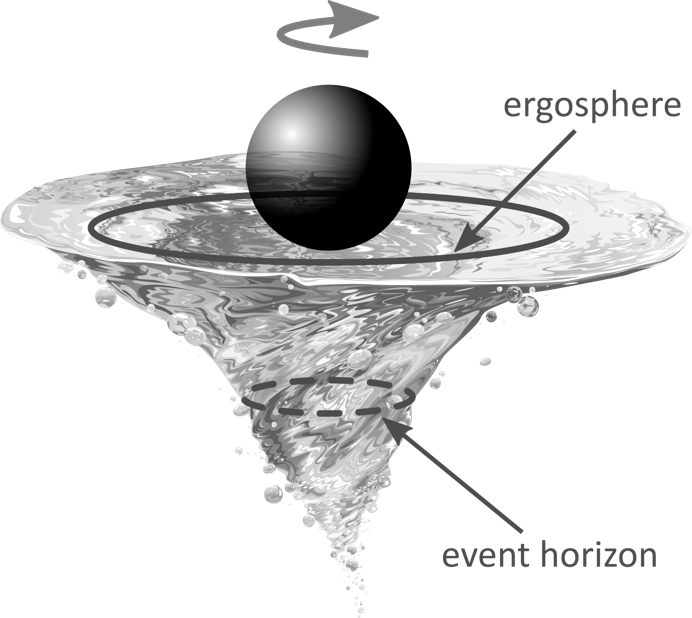
\includegraphics[width=0.88\linewidth,height=0.48\textheight,keepaspectratio]{../figs/source/en/fig-07-04.png}

% DOCX paragraph 927
\caption{\emph{Vortical motion of matter near a black hole and the position of the outer
edge of the ergosphere}\index{black hole!ergosphere}\emph{, which is clearly located at a radius
that is larger than that of the event horizon. © Jullands/depositphotos.com/LR.}}\label{fig:07-04}
\end{figure}

% DOCX paragraph 929
To give you some numbers, a Kerr black hole\index{black hole!Kerr} spinning almost at the
maximum rate allowed, i.e., with dimensionless spin \emph{a ≃ 1}, the event horizon is
set at a radius \emph{r\textsubscript{+}≃GM/c\textsuperscript{2}}, while the outer edge
of the ergosphere is at a radius that is almost twice as large,
\emph{r\textsubscript{0}≃2 (GM/c\textsuperscript{2})}.

% DOCX paragraph 930
Besides the forced corotation, the ergosphere is also a region near the black hole where
fascinating physical processes can occur. In particular, particles can be accelerated to
very high speeds, and the rotational energy\index{energy!rotational} of the black hole (i.e.,
its reducible mass) extracted with a mechanism called the ``Penrose
process\index{Penrose!process}'' (after the British physicist Roger
Penrose\index{Penrose!Roger}, who first described it in the 1970s).\textsuperscript{\hyperlink{note:07-05}{5}}
There is much that could be said on this very interesting topic, but that would move us
too far from our goal~\ldots{}

% DOCX paragraph 931
Instead, let's go back to our light rays and examine their trajectories near a rotating
black hole. Figure \ref{fig:07-05} describes this scenario, both in the case of a black hole
rotating clockwise (left panel) and a black hole rotating counterclockwise (right
panel). In both cases, the black holes are observed from above and, therefore, along the
axis of rotation.

% DOCX paragraph 938
\begin{figure}[htbp]
\centering
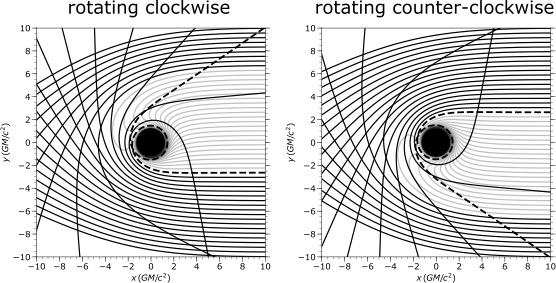
\includegraphics[width=0.88\linewidth,height=0.48\textheight,keepaspectratio]{../figs/source/en/fig-07-05.jpeg}

% DOCX paragraph 940
\caption{\emph{The same orbits as in Figure \ref{fig:07-03}, but related to rotating black holes.
The rotation of the black hole creates a vorticity in the trajectories, and the photons
must adapt to its direction of rotation. At the same time, the event horizon is
significantly smaller. © C. Fromm/LR.}}\label{fig:07-05}
\end{figure}

% DOCX paragraph 942
I think it is clear that the rotation of the black hole breaks the spherical
symmetry\index{spherical symmetry} present in Figure \ref{fig:07-03}, so the possibility of a
photon\index{photon!orbit} being captured by the black hole depends on which side it
approaches it. In particular, if it approaches from the side on which it is rotating
(for example, starting from negative values of the \emph{y} coordinate in the case of
the clockwise black hole), it will be easier for the photon to get very close to the
event horizon\index{event horizon} without being captured by it. In Figure \ref{fig:07-05}, this
phenomenon can be appreciated by considering the difference in the transition between
the black and grey lines around \emph{y=0}, or simply by comparing Figures 7.3 and 7.5.

% DOCX paragraph 943
Furthermore, when looking carefully at the two panels in Figure \ref{fig:07-05}, you can also notice
the presence of the ergosphere\index{black hole!ergosphere}. Just pay attention to the behaviour
of the photon orbits\index{orbit} approaching the black hole in the opposite
direction to that of rotation (for example, starting from positive values of the
\emph{y}-coordinate for the clockwise black hole). You can then see that, at a certain
point, the photons are forced to change their direction of motion and corotate with the
black hole\index{orbit!corotating}\index{photon!orbit}\index{photon!corotating}\index{photon!counter-rotating}.
Because the only difference between the right and left panels is in the sense of
rotation of the black hole, the two images are equivalent and antisymmetric. It is
possible to obtain one starting from the other by a simple rotation around the
\emph{x-}axis.

% DOCX paragraph 944
Note that what we have seen so far is only a small part of the general picture since our
attention has been restricted to photon orbits all lying in the same plane and, in
particular, in the equatorial plane of the black hole. However, the dynamics of light is
much more complex if we consider arbitrary photon orbits, that is, orbits not forced to
move on a precise plane. In this case, which represents the rule since only a small
fraction of the possible orbits is contained in a plane, the dynamics of light rays is
far more bizarre.

% DOCX paragraph 945
An example of a generic orbit\index{orbit!generic}, taken at random from millions I could
produce, is shown in Figure \ref{fig:07-06}. More specifically, it shows the trajectory of a photon
around a black hole that is rotating clockwise. The left panel offers a
three-dimensional reconstruction of the orbit, while the one on the right shows the
projections of the same orbit on two planes and serves to help us understand its
dynamics. Notice how the orbit is considerably more complex (but I guarantee there are
even more complex ones) and how the photon can get very close to the black hole, making
at least four revolutions without being captured. In the end, it is deflected in a
direction that is almost diametrically opposed to the initial direction. Furthermore,
since the orbit refers to a photon not absorbed by the black hole, it is symmetric under
``time reversal\index{time reversal}''. In other words, it doesn't matter which end you
start from when following it, since it can be walked both ways.

% DOCX paragraph 946
\begin{figure}[htbp]
\centering
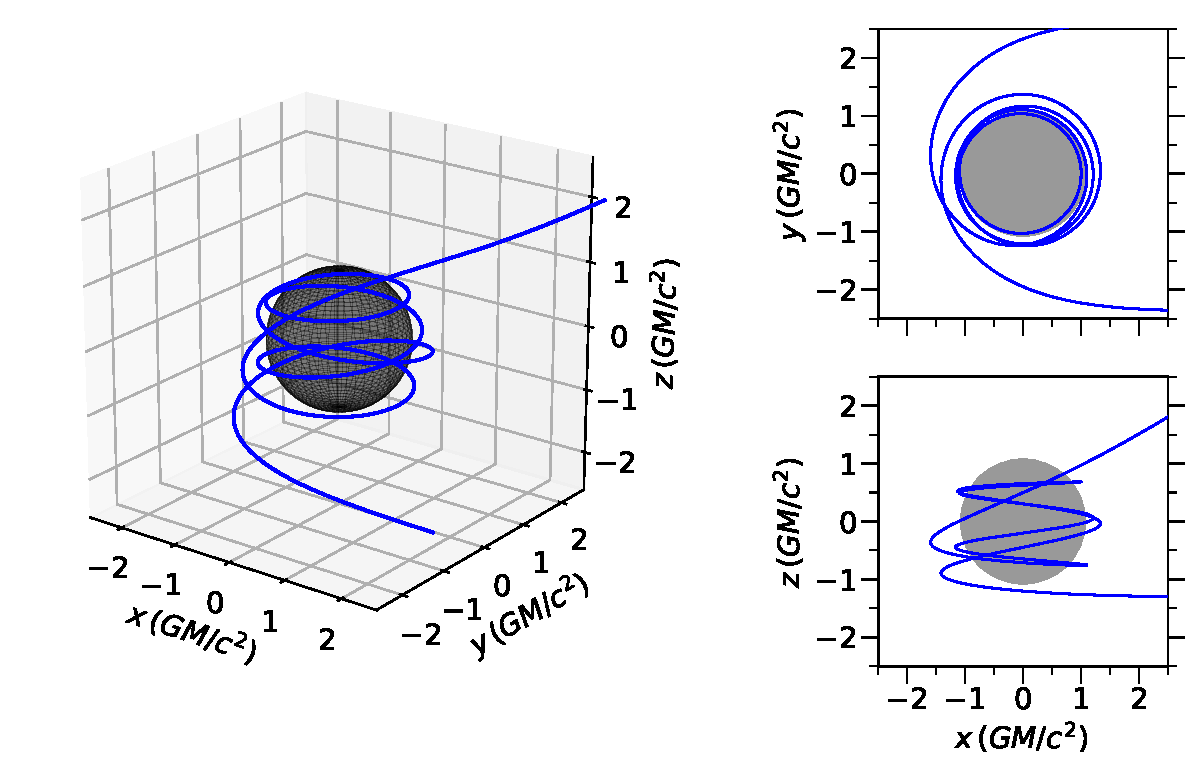
\includegraphics[width=0.88\linewidth,height=0.48\textheight,keepaspectratio]{../figs/pdf/en/fig-07-06.pdf}

% DOCX paragraph 948
\caption{\emph{Generic orbit of a photon around a rotating black hole. © C. Fromm/LR.}}\label{fig:07-06}
\end{figure}

% DOCX paragraph 950
As already mentioned, the complexity of the trajectory shown in Figure \ref{fig:07-06} is not an
exception but rather the rule. It is enough to modify the initial conditions slightly to
obtain countless equally complex and intriguing variants. This property has important
implications for what we will see later when I discuss how the EHT image of
M87*\index{M87*} was ``produced'' from the observations. However, if the dynamics
of light near a black hole can be so complex, and a photon coming from one direction can
go back in the same direction it came from (not something we are at all used to in our
flat-spacetime experience!) then, reconstructing an image from all these orbits will be
highly complicated. Indeed, suppose that light can be emitted and received from any
direction. Then, one may even fear it is impossible to obtain a coherent photo of the
regions close to a black hole or that the corresponding images will be indistinct
smudges of intensity devoid of detail. However, the radiation is not emitted everywhere,
only in specific regions and part of the emitted radiation is absorbed by the black hole
and doesn't reach us. This makes for a compelling display of lights and shadows that
combine to produce an image that, in realistic astrophysical conditions, has very
particular properties, as we will see.

% DOCX paragraph 953
\section{A Game Of Lights And Shadows}\label{sec:07-shadow}

% DOCX paragraph 955
We have just seen how complex the trajectory of light rays can be in a curved spacetime
and, in particular, near a black hole. We have even learnt that a photon can go back to
where it was emitted. These behaviours are very different to those we are familiar with
on Earth, where light essentially travels in a straight line and we see what is in front
of us, certainly not what is behind us. Furthermore, if we have an object in front of
us, we can receive its direct image and not an indirect image of what is behind it. Just
think how surprising it would be if, approaching a man in a suit and tie, you could also
see a stain on his back. Well, all this is possible in the vicinity of a black hole!

% DOCX paragraph 956
To further complicate matters, we have to consider that light not only changes direction
but can also ``disappear'' when captured by the black hole. To cut a long story short,
it is clear that to understand what happens to light in the vicinity of a black hole,
and if we want to know what to expect, we must re-educate our
perception\index{perception} of what is possible or impossible in extreme conditions of
curvature. In particular, we will now consider precise geometric shapes that correspond
to potential light sources around a black hole and deduce how an observer at an
astronomical distance will see them. We will thus discover that a considerable fraction
of light rays can disappear to create dark areas, or ``shadows'', but can also be
concentrated and amplified as if through a lens.

% DOCX paragraph 957
Figure \ref{fig:07-07} shows the simplest scenario to consider, one that allows us to appreciate
some of the subtleties of producing an image of an object in the vicinity of a black
hole. This figure illustrates a nonrotating and isolated black hole (without matter
around it) whose event horizon\index{event horizon} appears as a small grey sphere. The
black hole is in front of a light source, for example, a beautiful starry sky,
represented very schematically in the left part of the diagram. The aim is to understand
what happens to a beam of light emitted by this source and how it is received by a
distant observer on the right of the image.

% DOCX paragraph 959
\begin{figure}[htbp]
\centering
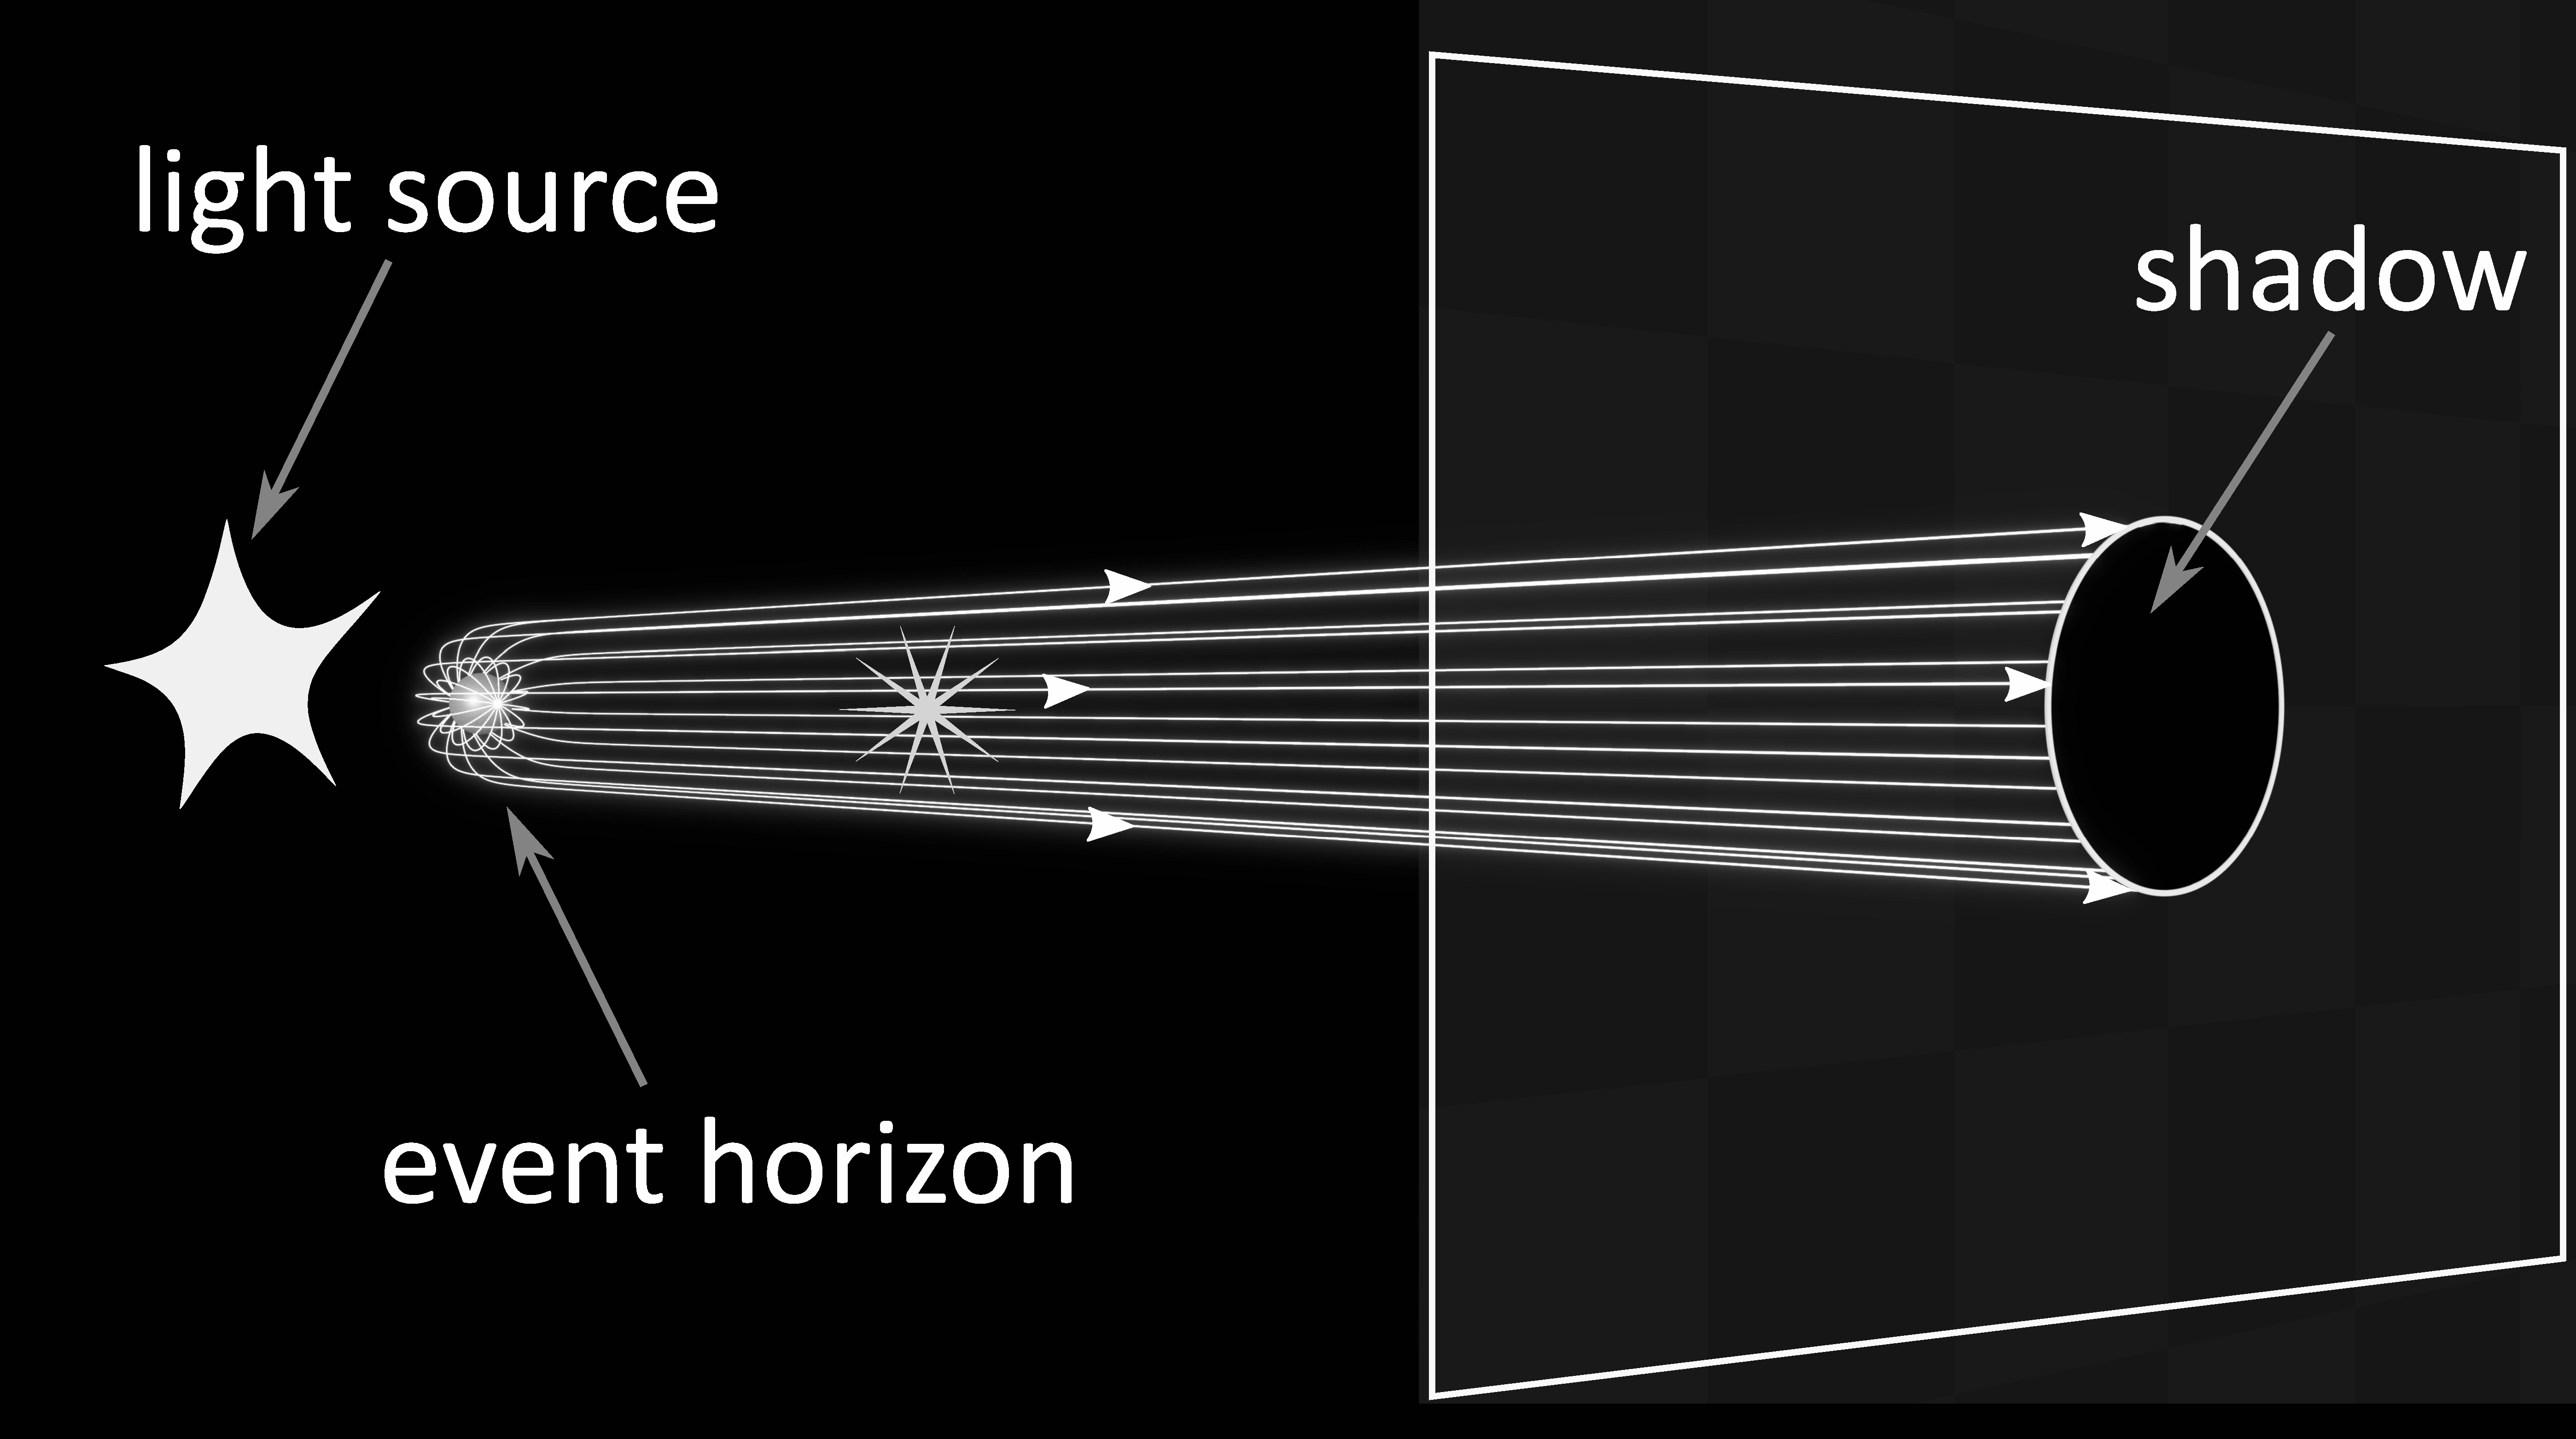
\includegraphics[width=0.88\linewidth,height=0.48\textheight,keepaspectratio]{../figs/pdf/en/fig-07-07.pdf}

% DOCX paragraph 961
\caption{\emph{Creation of a ``shadow}\index{shadow (black hole)}\emph{'' of a black hole. © T.
Müller/M. Pössel (MPIA)/LR.}}\label{fig:07-07}
\end{figure}

% DOCX paragraph 963
At this point, you should have a fairly clear idea of what happens to a beam of light
shot at a black hole, and you should be able to imagine what a distant observer would
see in their sky. The black hole will immediately absorb a proportion of the photons
emitted by the source, that is, those whose trajectory intersects the spherical surface
of the event horizon. Conversely, other photons will not intersect the event horizon but
pass close enough to be deflected and captured by the black hole. The margin of the
trajectories that will ``escape'' the capturing power of the black hole is given by the
unstable photon circular orbit, or light ring. Hence, an observer at large distance will
see an area almost devoid of light as the black hole has intercepted all the
photons\index{photon!shadow} that should have reached them. Therefore, what will be seen,
is the ``shadow'' of the black hole\index{shadow (black hole)}.

% DOCX paragraph 964
The basic and yet fundamental phenomenon just described leads us to three considerations
helpful in removing some urban legends or incorrect ideas about black-hole shadows. The
first is that observing the shadow does not mean we observe the event horizon. The
shadow is, in fact, determined not only by the photons that hit the event horizon
directly but also by those that approach it at a distance less than the light ring.
Furthermore, since it is an image projected onto the sky, it is necessarily larger even
than the light ring itself. To be precise, the edge of the shadow\index{shadow (black hole)},
and therefore its size, is defined as the impact parameter of the unstable circular
orbit of photons\index{orbit!unstable circular (photon)}\index{photon!unstable circular orbit}, and its radius for a nonrotating
black hole is given by
\emph{r\textsubscript{sh}=}\(\sqrt{27}\)\emph{(GM/c\textsuperscript{2})}. Since
\(\sqrt{27} \simeq 5.2\), the shadow (the darkest part in the centre of the image in
Figure \ref{fig:07-01}) is larger (by almost three times) than the event horizon\index{event horizon}
\emph{r\textsubscript{S}=2(GM/c\textsuperscript{2})}. Moreover, the size of the shadow,
just like the event horizon, is proportional to the mass of the black hole, so the more
massive a black hole, the larger its image in the sky, and the easier it is to take a
picture of it at a given distance.

% DOCX paragraph 965
The second important consideration is that the shadow represents an area in the sky
where some light is ``missing'', i.e., the light absorbed by the black hole. However,
this area does not have to be totally devoid of light. Only the event horizon cannot
emit light, so it is perfectly normal that the area corresponding to the shadow also
contains some radiation. For instance, a photon emitted by a source located between the
event horizon and a distant observer, such as the little white star in Figure \ref{fig:07-07}, would
not be absorbed by the black hole if directed towards the observer. For this reason, the
shadow in the image of M87*\index{M87*} in Figure \ref{fig:07-01} is not perfectly dark. The
EHT has actually used the contrast in the intensity between the centre of the image and
the bright ring to constrain the properties of M87*.

% DOCX paragraph 966
The third and final consideration is that, with the exception of a nonrotating black
hole, in which case the spherical symmetry\index{spherical symmetry} ensures that the
shadow\index{shadow (black hole)} is always the same (a perfect circle), the shape of the shadow
will depend both on the spin of the black hole and on the inclination with respect to
the axis of rotation at which the observations are made. This is because, as anticipated
above, the rotation of the black hole generates a rotation of the entire spacetime in
its vicinity (i.e., the frame-dragging effect), which allows photons that approach the
black hole from one side to get closer to the event horizon than those on the opposite
side (see Figure \ref{fig:07-05}).

% DOCX paragraph 967
The presence of rotation, and thus the loss of spherical symmetry\index{spherical symmetry},
also has another consequence: the shadow can change its appearance when viewed from
different angles. In particular, the shadow of a rotating black hole will appear
perfectly circular if observed along the polar direction (i.e., if we looked at it from
the North Pole or the South Pole). In contrast, it would appear deformed when viewed
from the equatorial plane.

% DOCX paragraph 973
\section{Shadows And Discs}\label{sec:07-discs}

% DOCX paragraph 975
Because the shape of the shadow\index{shadow (black hole)} depends on the spin of the black
hole, it is possible, at least in principle, to deduce the spin of the black hole by
``simply'' measuring the shape of the shadow observed. In reality, things are much more
complicated than in this simplified description and measuring the shape of the shadow
with precision is still extremely difficult given the current accuracy of the
observations. Essentially, it is for this reason that the observations made by the EHT
on M87*\index{M87*} have not been able to provide a measure of its spin, even
though it is improbable it is a Schwarzschild black hole\index{black hole!Schwarzchild}. We will
come back to this point when we talk about comparing the observations and predictions of
the theory.

% DOCX paragraph 976
Setting aside the enormous technical difficulties that still need to be overcome to
obtain a sharp image of the shadow, its shape remains a formidable tool for
understanding the properties of the black hole. However subtle, all the information
about mass, spin and charge (the only three properties of a black hole) are imprinted on
its shadow. I find the fact we can shed light on black holes by simply measuring how
they mark the absence of light as fascinating as it is paradoxical. This is true in
general and applies not only to black holes in general relativity but to black holes in
alternative theories and also to compact objects that aren't even black holes! We will
return to these considerations when we ask ourselves whether M87*\index{M87*}
really is a black hole~\ldots{}

% DOCX paragraph 977
Awaiting us now is an important qualitative leap in the understanding of the features
that a realistic image of M87*\index{M87*} should have. Everything discussed so
far, in fact, refers to the highly idealised physical conditions of an isolated black
hole in front of a background of light-emitting sources. Under realistic astrophysical
conditions, however, a black hole will be surrounded by plasma at high temperatures and
energies, which is falling onto it in the form of an accretion disc. So, what does a
black hole look like under such conditions?

% DOCX paragraph 978
The short answer is that it will look very different from what we might expect in a flat
spacetime. However, to get to the long answer, we need to proceed once again through an
idealisation. So, instead of considering the image produced by a realistic accretion
disc, whose properties result from sophisticated numerical simulations, let's first
model the disc with a simpler geometric shape. This will help us understand some of the
most salient properties of the gravitational lensing effects (the distortions in an
image due to a curved spacetime) that characterise the image of an accretion disc around
a black hole.

% DOCX paragraph 979
Let's, therefore, consider an accretion\index{accretion disc!thin} disc made of a vertically
thin ring of matter centred around the black hole. In other words, let's imagine putting
a very thin doughnut around a black hole and asking ourselves how would the doughnut
appear to us if we were to observe it from a large distance and at a certain angle.

% DOCX paragraph 980
This is just what Figure \ref{fig:07-08} shows, where we see, on the left, a black hole surrounded
by a thin disc of matter, and, on the right, the image received by an observer placed at
a certain angle of inclination. However, an important difference between this figure and
Figure \ref{fig:07-07} is that the black hole is now not illuminated by an extended source behind
it. Instead, the accretion\index{accretion disc!thin} disc itself acts as a source of light, and
therefore it can appear deformed by the distortion of the trajectories of light around
the black hole.

% DOCX paragraph 981
\begin{figure}[htbp]
\centering
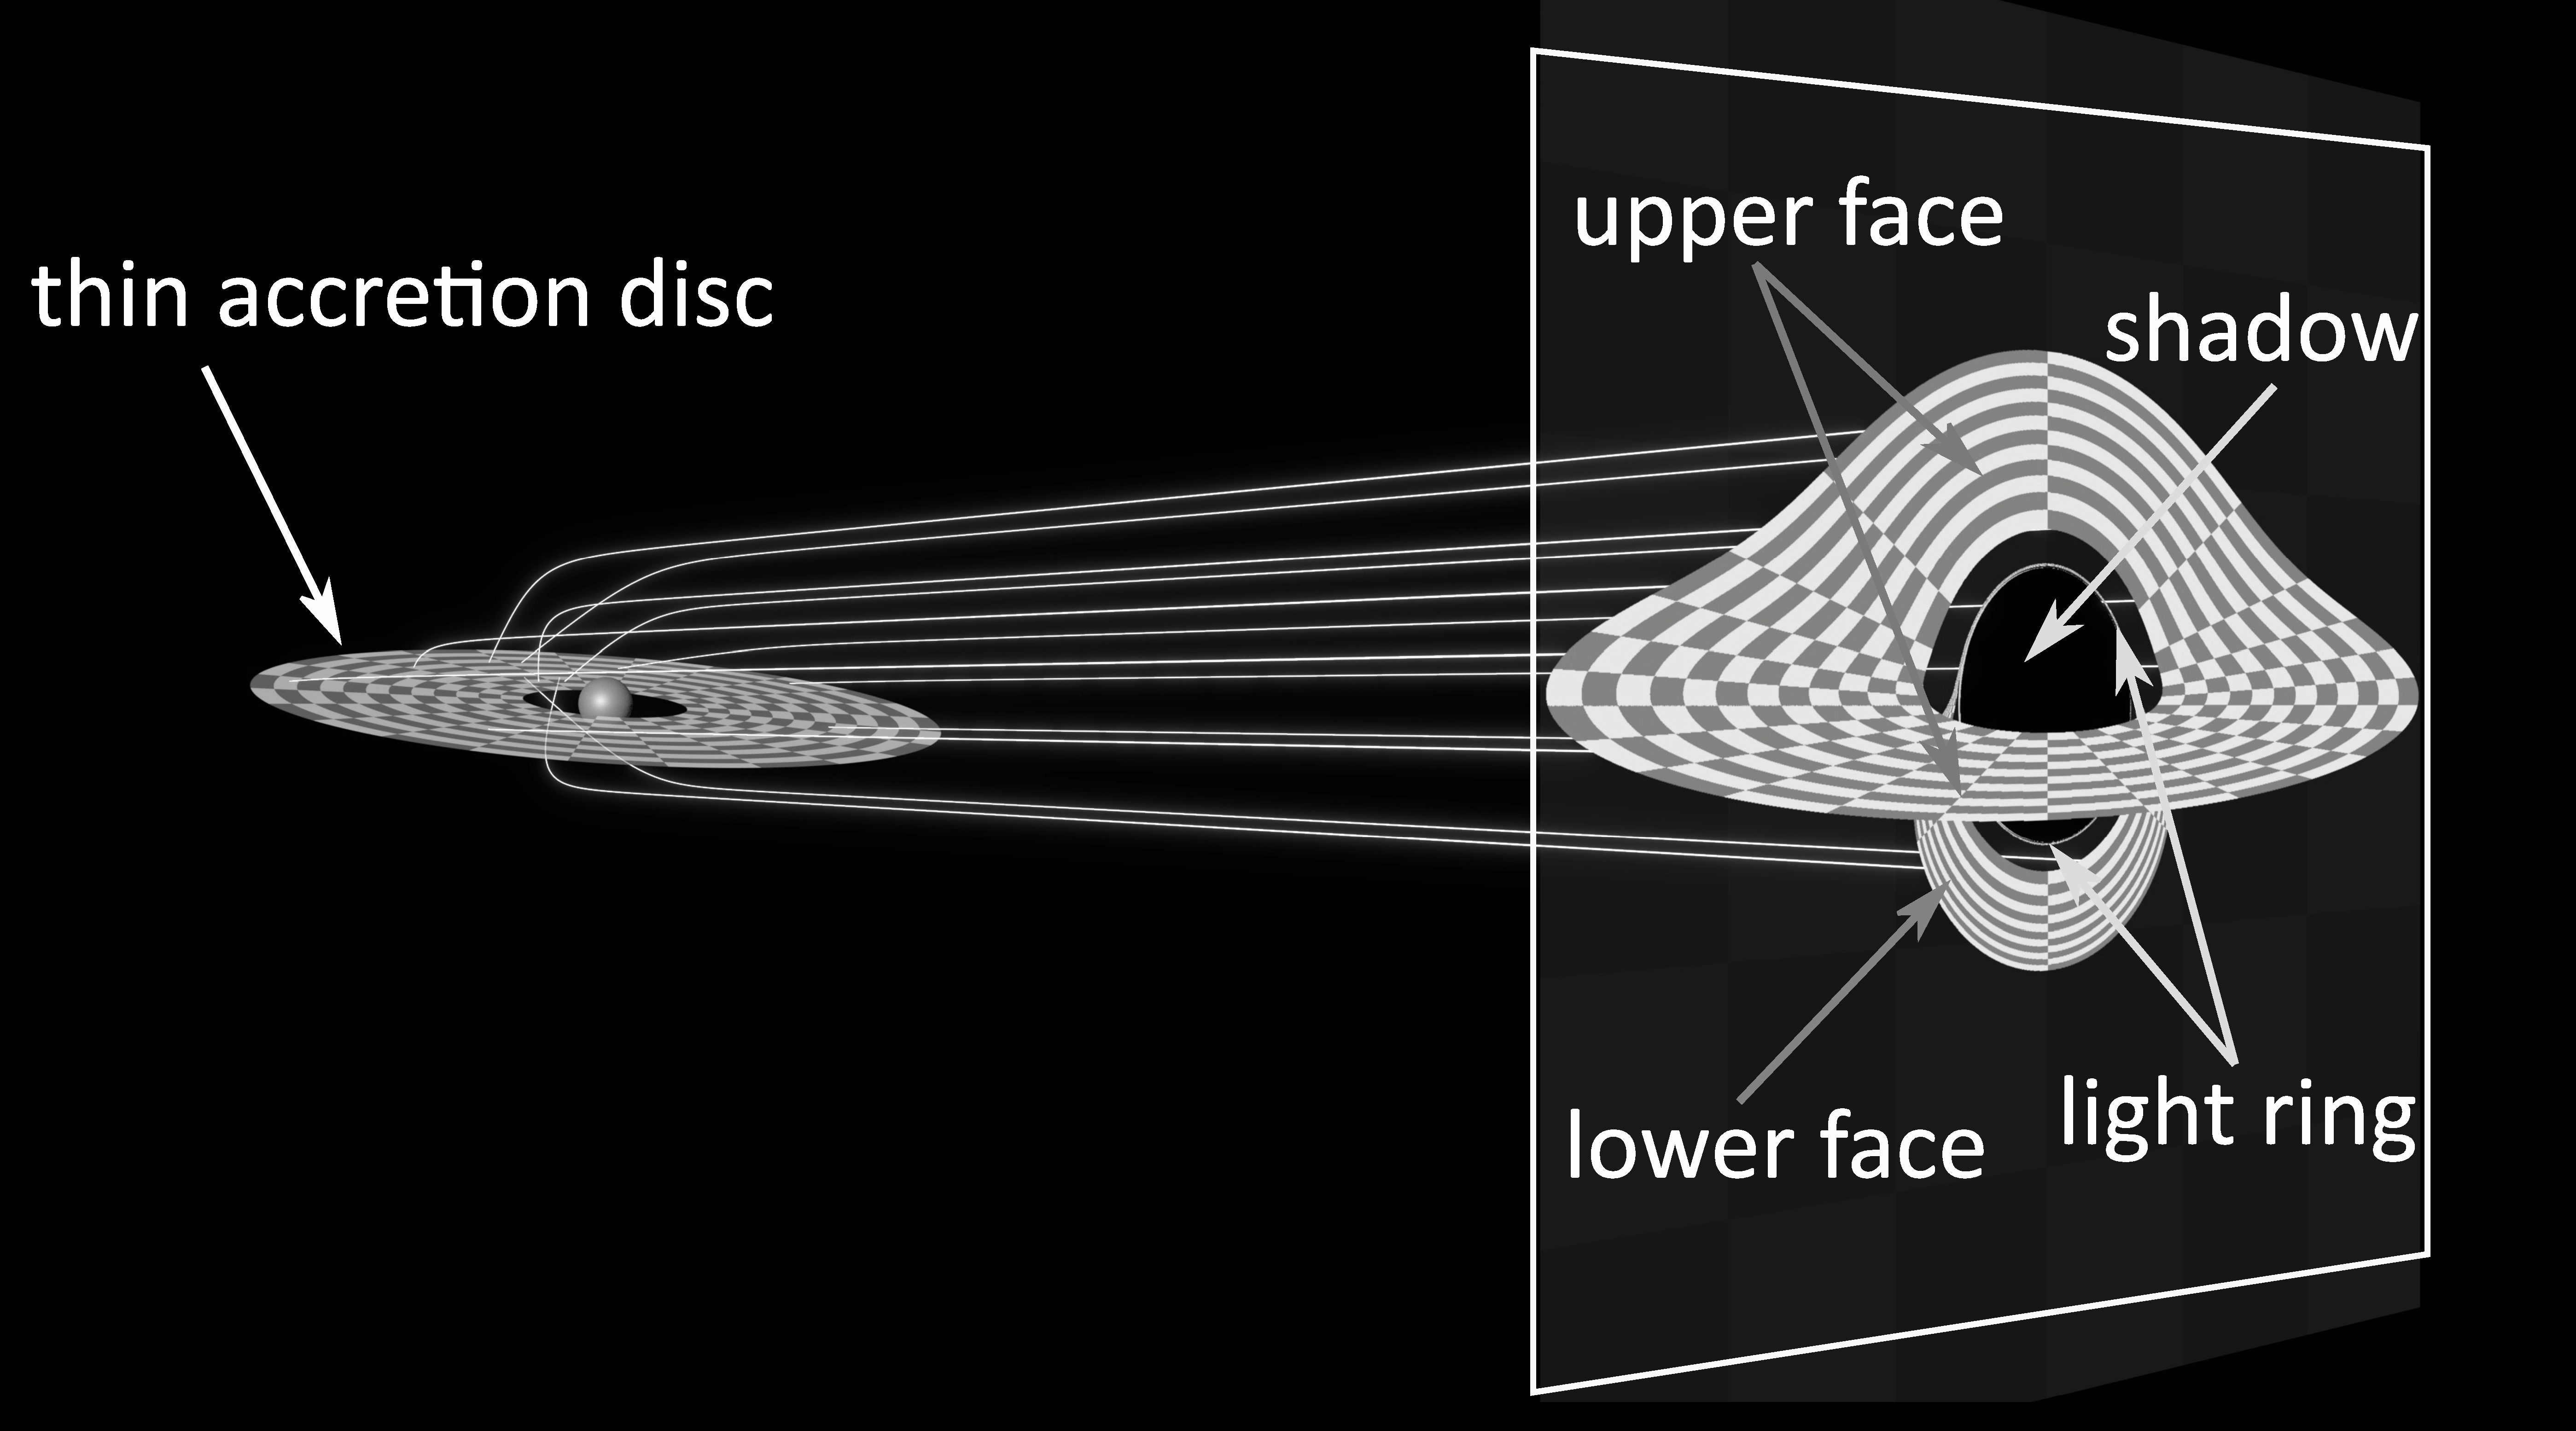
\includegraphics[width=0.88\linewidth,height=0.48\textheight,keepaspectratio]{../figs/pdf/en/fig-07-08.pdf}

% DOCX paragraph 983
\caption{\emph{How a very thin accretion disc would appear to a distant observer. © T.
Müller/M. Pössel (MPIA)/LR.}}\label{fig:07-08}
\end{figure}

% DOCX paragraph 985
Clearly, in a flat spacetime\index{spacetime!flat}, we would see only the portion of the
disc that is closer to us, that is, the front part of the upper face of the disc, as
this is the portion of the disc from which photons\index{photon} moving on a
straight line can reach our eyes. However, since the disc is in a region of very curved
spacetime, the resulting image is rather different! In particular, Figure \ref{fig:07-08} shows how
the ``doughnut'' is very distorted. Not only would we see the front part of the upper
face of the disc, but also the back part of the upper face, that is to say, the part
behind the black hole and that we, therefore, wouldn't be able to see in a flat
spacetime. Admittedly, this is a bizarre effect but perfectly normal in a curved
spacetime. Furthermore, it teaches an important lesson: if you find yourself in outer
space and need to hide, well, don't go behind a black hole! It would be totally
pointless and just reveal how unfamiliar you are with general relativity~...

% DOCX paragraph 986
The bizarreness doesn't stop there. The curvature of spacetime would be such that we
could also see the lower face of the back part of the disc, which would appear to us in
the lower part of the image as a hanging appendage. In essence, we would see almost
every part of the disc. It is important to note that the shadow\index{shadow (black hole)} would
not be a single darker region but would be split into two parts: one visible above the
top face of the disc and one below it. Finally, it would be possible also to observe the
light ring, which in Figure \ref{fig:07-08} is represented by a very thin ring; despite its
thinness, it would appear relatively bright since spacetime can focus a large number of
photons on this ring.

% DOCX paragraph 987
Those of you who love science-fiction movies as much as I do (especially ones with a
healthy dose of realism and physical consistency) may have recognised the image of the
accretion disc on the right of Figure \ref{fig:07-08}, which closely resembles the supermassive
black hole \emph{Gargantua,} which stars in Chris Nolan\index{Nolan, Chris (Interstellar)}'s movie
``\emph{Interstellar}'' (2014). This is no coincidence; the representation of Gargantua
in ``Interstellar'' is, in fact, quite realistic, even though it does contain at least
two unrealistic aspects.

% DOCX paragraph 988
The first is that the accretion disc around Gargantua is shown as being geometrically
thin, that is, with a very small vertical height. In reality, the physical conditions of
the accreting plasma\index{plasma!accreting} near a supermassive black hole lead to very high
temperatures and pressures inside the accretion disc, forcing it to ``inflate'',
especially in the regions closer to the black hole. As a result, a realistic
accretion\index{accretion disc!thick} disc is actually geometrically thick, with a non-negligible
vertical height, as shown by the various images in Figure \ref{fig:07-09}. More specifically, the
four panels show four different examples of a realistic accretion\index{accretion disc!thick}
disc emitting radiation at a radio frequency of 230 GHz computed from a sophisticated
numerical simulation. The inclination angle of a distant observer differs in the various
images, as indicated by the symbol at the bottom right of each panel, which also shows
the direction of rotation of the plasma.

% DOCX paragraph 989
In particular, let's focus on the panels on the top left and the bottom right of Figure
\ref{fig:07-09}. Both represent quite generic situations and show how a realistic accretion disc
would appear as more ``fluffy''. But, the basic features discussed in Figure \ref{fig:07-08} remain
valid, namely, the possibility of seeing both faces of the disc and the doubling of the
shadow\index{shadow (black hole)}.

% DOCX paragraph 990
\begin{figure}[htbp]
\centering
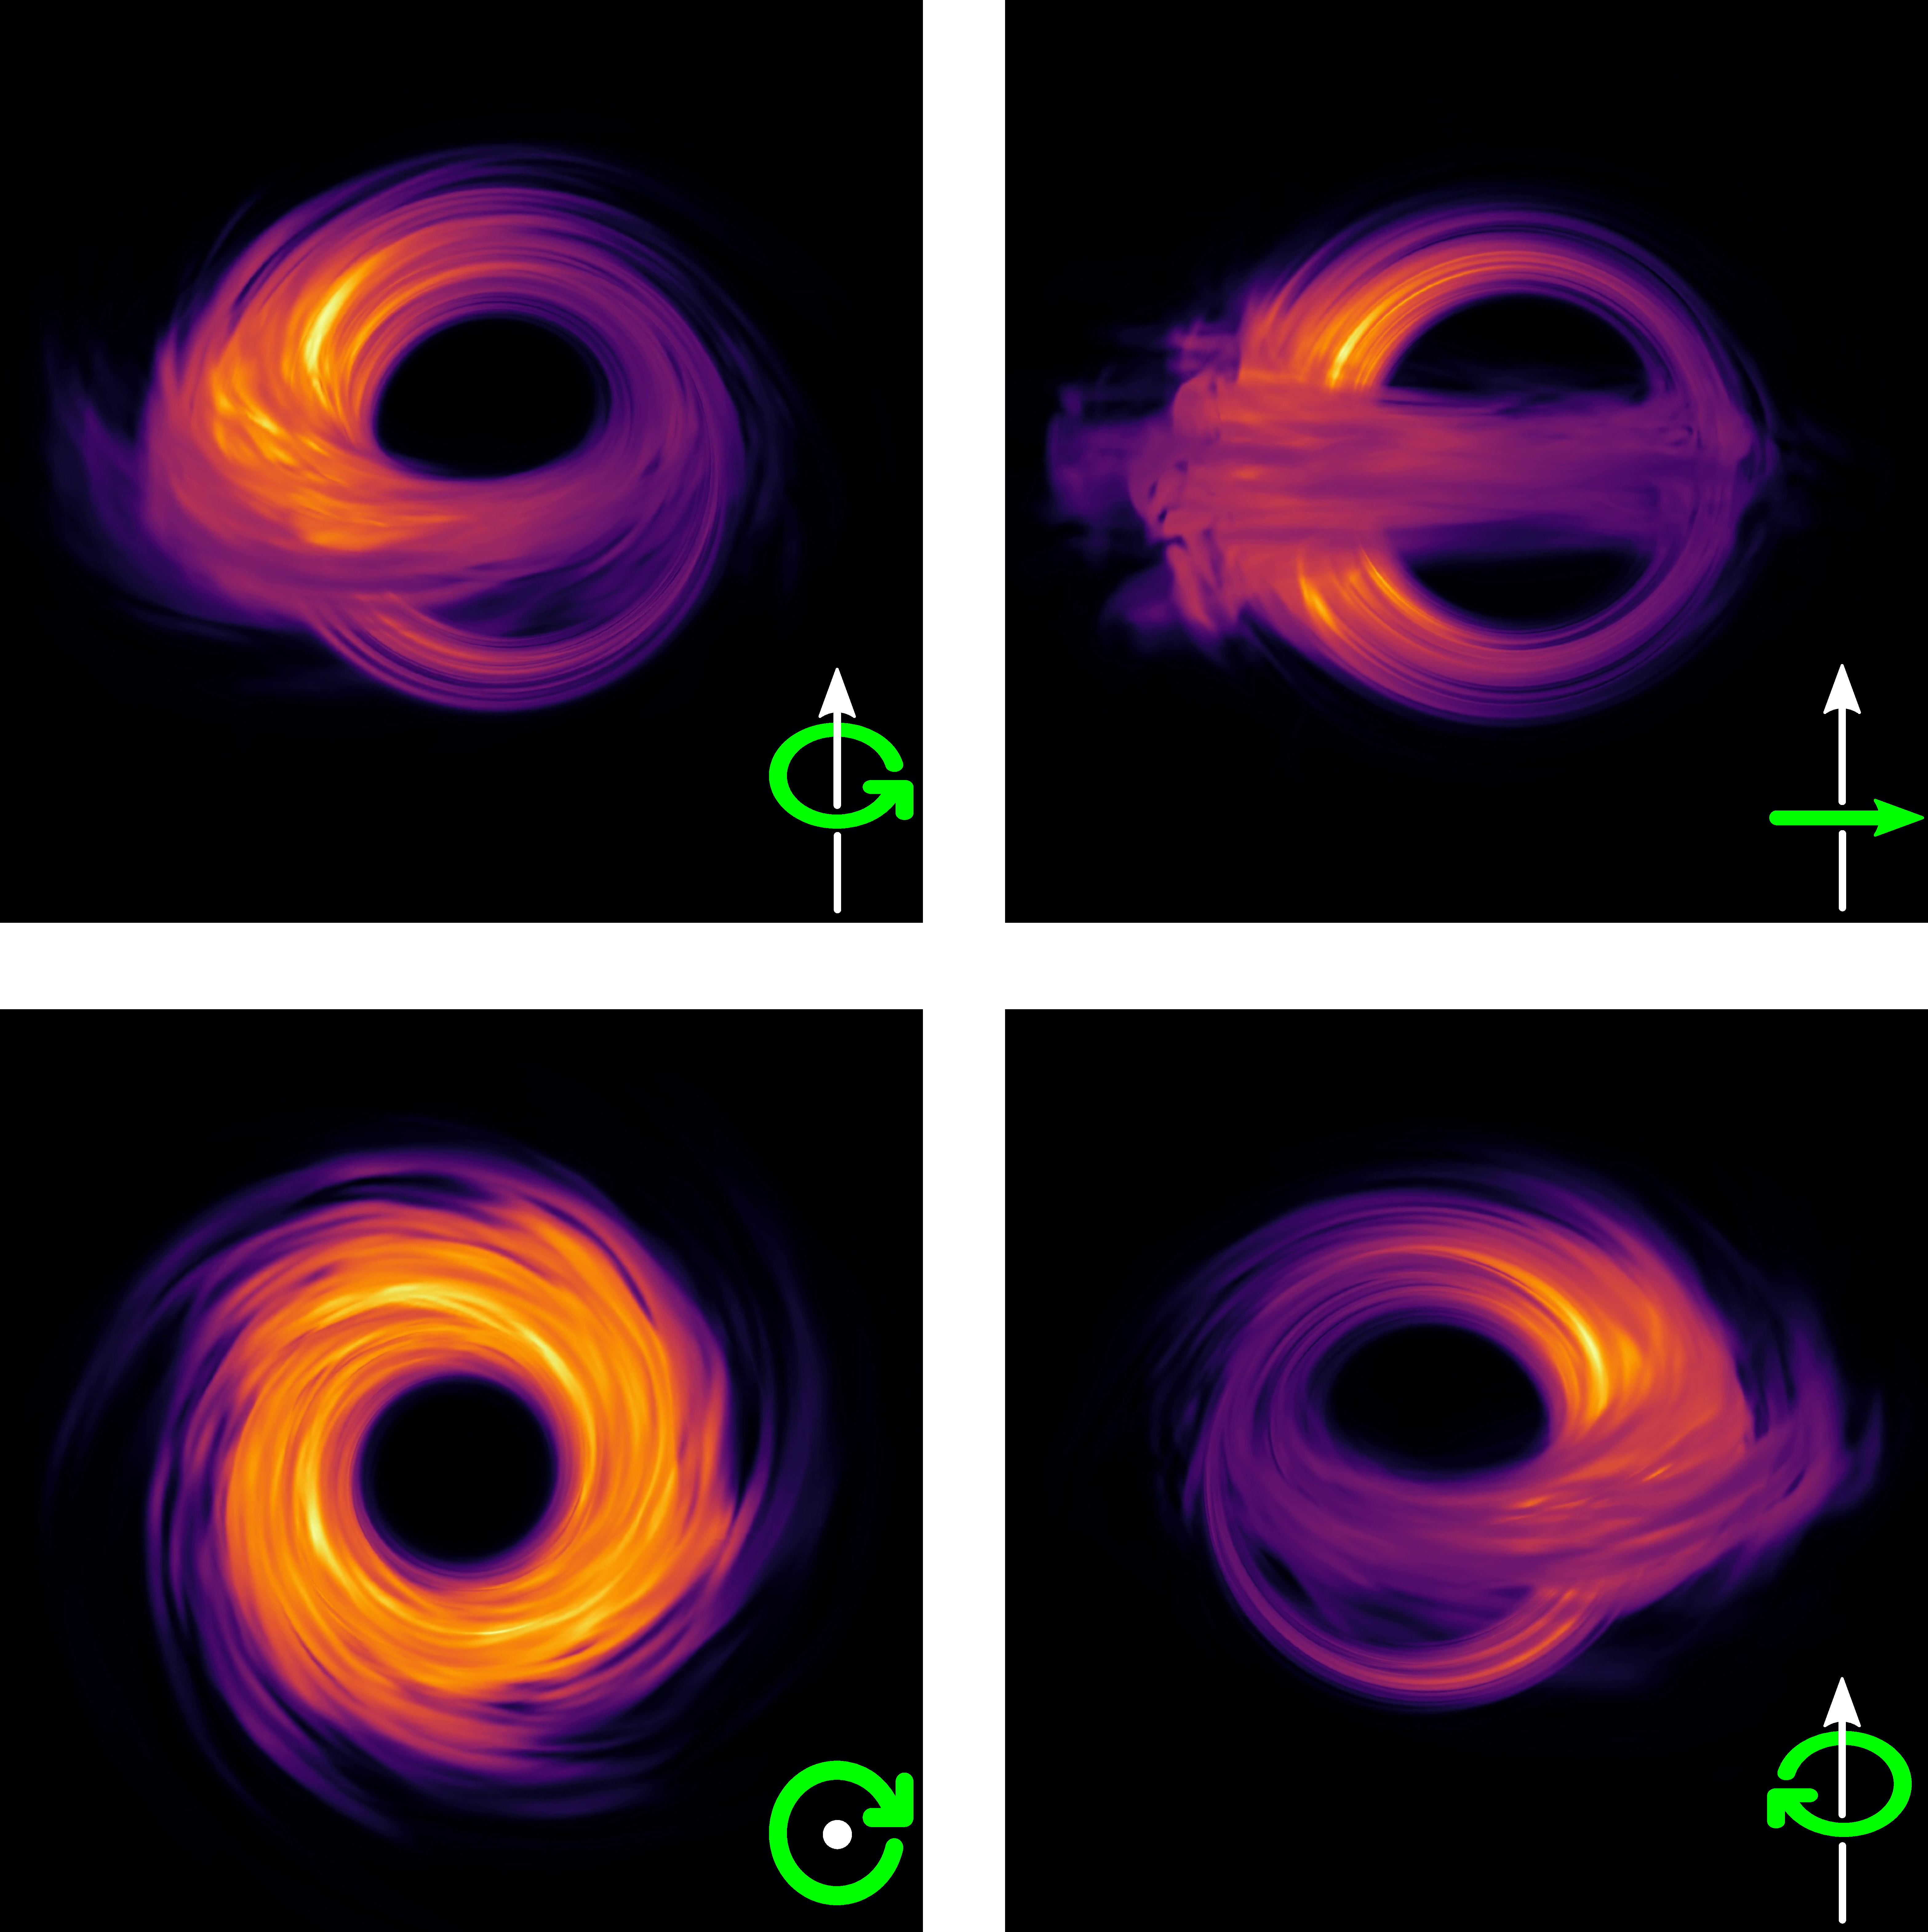
\includegraphics[width=0.88\linewidth,height=0.48\textheight,keepaspectratio]{../figs/pdf/en/fig-07-09.pdf}

% DOCX paragraph 992
\caption{\emph{Different angle images of a thick accretion disc around a rotating black
hole. © Z. Younsi/LR.}}\label{fig:07-09}
\end{figure}

% DOCX paragraph 994
The second important aspect, shown in the panels of Figure \ref{fig:07-09} and absent in the image
of the disc around Gargantua, is that all discs have a side that is brighter and,
consequently, a side that is less bright. The only exception, which I have decided to
show precisely because it is an exception, is illustrated in the bottom left panel and
refers to the case of a zero inclination (i.e., when viewing the accretion disc from the
direction of the North Pole). The origin of the asymmetry in the brightness between the
two sides of the disc is linked to a common phenomenon, the Doppler
effect\index{Doppler!effect} (after the Austrian physicist who first described it in 1842).
This effect is responsible for the variation of the frequency of a wave signal when
emitted by a moving source. In other words, it describes the well-known variation in
frequency of an ambulance's siren as it moves towards or away from us. We have all
experienced an ambulance approaching us and the frequency of its siren increasing in
what is known as a ``\emph{blue-shifted}'' \index{blue-shift (Doppler)}Doppler signal. For the
same reason, the siren's frequency decreases as the ambulance moves away from us,
producing what is described as a ``\emph{red-shifted}'' \index{red-shift (Doppler)}Doppler
signal.

% DOCX paragraph 995
Although the Doppler effect is already present in classical physics, and we experience
it routinely for sources that move at low speeds in respect to us, it takes on new
relevance in relativity, as the emission changes not only in frequency but also in
amplitude. More specifically, the signal emitted by a source moving towards us at speeds
close to that of light will be both shifted towards the blue and amplified in intensity.
The amplification, which is particularly large for speeds of the source close to that of
light, is usually referred to as the relativistic Doppler
\emph{``boost}''\index{Doppler!boost}\index{relativistic!Doppler effect}.

% DOCX paragraph 996
Returning to Figure \ref{fig:07-09}, the reason three of the panels have a ``bright side'' is that,
in all three, there is matter that rotates around the black hole, so there is a side in
which matter moves towards us and its brightness is, therefore, amplified by the
relativistic Doppler boost.\textsuperscript{\hyperlink{note:07-06}{6}} For the same reason, matter on the
opposite side of the disc is moving away from us, and the corresponding emission is
suppressed. This also explains why the bottom left panel in Figure \ref{fig:07-09} does not have a
bright side or a dark side. For such inclination, there is no area of the disc that
moves towards us (all motion is in a plane perpendicular to our line of sight) and,
therefore, there is no part of the accretion disc whose emission can be amplified in any
way.

% DOCX paragraph 999
\section{The Predictions Of The Theory}\label{sec:07-theory}

% DOCX paragraph 1001
We have seen how the radiation emitted in the vicinity of a black hole can be subject to
incredible tricks of light and shadows\index{shadow (black hole)}. We have also seen how an
object with a disc geometry (be it thick or thin) emitting radiation in the radio band
may appear radically different from what we would expect of our experience in flat
spacetime. What remains to be seen and understood is what the physical properties of
this emitting object should be. In other words: ``What happens to matter near a
supermassive black hole?''.

% DOCX paragraph 1002
An easy way to answer this question would be to take a certain amount of matter, such as
a large bucket of water, and throw it over a rotating black hole. We could thus observe
what happens to the matter as it falls on the event horizon and use the data obtained to
infer what generally happens to accreting matter on a supermassive black hole.

% DOCX paragraph 1003
Sure, it would be very convenient to be able to do this, and it would solve a lot of
problems for me personally, even though, in all likelihood, it would leave me
unemployed. However, it is obvious, unfortunately, that this path is not viable. So, the
only way (and I must emphasise the ``only'' way) to answer this question is to take the
equations that describe the behaviour of water poured onto a black hole and solve them
with the help of powerful supercomputers\index{supercomputers}. I have learned to do
exactly this ever more realistically throughout my scientific career.

% DOCX paragraph 1004
I am well aware that when I say I make a living solving partial
differential\index{differential!equations} equations involving black holes and neutron stars, I am
widening the gap between myself and my interlocutors. To avoid doing this with you, I
will try to explain what this amounts to by using an analogy I am sure you are familiar
with. Solving differential equations to understand what happens to matter in the
vicinity of a black hole is, albeit with some differences, similar to what is done to
obtain weather forecasts. For many of you, a weather forecast\index{weather forecast} boils
down to a series of icons on a website or a geographic map with symbols representing
rain, clouds or sunshine, illustrated by a presenter on television. In reality, however,
those icons and symbols on the map are the results of complicated calculations made
several times a day, using parallel supercomputers\index{supercomputers} that solve the
equations of classical viscous hydrodynamics (also known as the
Navier-Stokes\index{Navier-Stokes equations} equations). It is no coincidence that these are also
partial differential\index{differential!equations} equations. In other words, the supercomputers
start with fairly precise information (collected by ground-based stations or airline
pilots) about the weather conditions, such as the wind speed, temperature, or the
density and composition of the atmosphere in different locations. These pieces of
information form the ``initial conditions'' and are then used to solve the
Navier-Stokes\index{Navier-Stokes} equations on a given region with a given angular
resolution\index{angular resolution}. In this way, it is possible to obtain predictions for the
velocity, temperature and density distributions of the atmosphere in the future. This
whole complicated process is summarised as ``weather predictions'', which somewhat
trivialises it. In reality, what we obtain is the solution of beautiful and complex
equations, once again evidence that mathematics pervades our world more deeply than it
may appear at first sight.

% DOCX paragraph 1005
Well, together with my colleagues, what I do is rather similar, at least in principle.
I, too, have to start from the initial conditions (for example, the quantity of water in
the bucket poured onto the black hole and its composition) and solve equations that tell
me where that water goes, if it remains as it is, or whether it vaporises into an
ionised plasma. The equations I am dealing with are those of general relativistic
magnetohydrodynamics\index{relativistic!magnetohydrodynamics} (which describe the dynamics of a
plasma\index{plasma} in the presence of intense magnetic fields and strong
spacetime curvature). And, I do not deny that they are much more complex than those used
in weather forecasts to compute the cloud coverage of a particular geographical area.
The physical regimes in which these equations are solved are also much more extreme,
with variations in temperature and densities that are the most severe
imaginable.\textsuperscript{\hyperlink{note:07-07}{7}}

% DOCX paragraph 1006
Notwithstanding these (important) differences, and at the risk of oversimplifying
things, it is possible to say that what we do in our simulations of plasma dynamics is
not so different from weather forecasting. Clearly, our simulations are not aimed at
predicting the weather in the vicinity of a black hole but at establishing what happens
to the matter that has found itself, for various reasons, orbiting the black hole.

% DOCX paragraph 1007
Thus, the simulations tell us that the plasma does not accrete onto the black hole in a
spherically symmetric manner; that is to say, it does not build up a single spherical
cloud in which the plasma falls onto the black hole following radial trajectories.
Rather, it concentrates on a plane referred to as the ``equatorial plane'', forming a
disc that rotates around the black hole while accreting onto it. The simulations also
reveal that the accretion disc around a supermassive black hole such as
M87*\index{M87*} cannot be geometrically thin, as portrayed in the
``Interstellar'' movie. Instead, it must have the shape of a thick doughnut and,
moreover, a doughnut that is neither stationary nor perfectly symmetric. Numerous
processes and instabilities driven by the strong magnetic fields develop in the
accretion disc and are responsible for dissipation and the ultimate falling of the
matter onto the black hole.

% DOCX paragraph 1008
The nice thing about numerical simulations is that they give us access to all the
properties of the plasma, such as density, velocity, temperature, and pressure. In this
way, we can calculate how much matter falls into the black hole per unit of time
(technically referred to as the ``accretion rate'') or how strong the magnetic field is
near the event horizon. Through the simulations, we discover, for instance, that the
accretion rates of both matter and magnetic field are not steady over time but are
``quasi-stationary''; that is, they fluctuate around some average value that remains
only approximately constant over time. Not very different to what happens to the water
falling from a waterfall: the amount of water falling per unit of time is only
approximately constant, accompanied by fluctuations associated with times in which there
is either more or less water falling.

% DOCX paragraph 1009
Finally, the simulations reveal that the accretion process inevitably leads to the
development of ``relativistic jets'' \index{relativistic!jet} in the polar areas of the black
hole. That is to say, regions where there is very little matter (almost as if there was
a vacuum\index{vacuum}), but where magnetic fields are instead very strong. Indeed,
magnetic fields are the dominant force in these jets and essentially determine the
dynamics of the plasma. Because of the underlying symmetry in the accretion process,
these jets normally come in pairs, with the magnetic field essentially aligned in a
direction perpendicular to the equatorial plane of the disc. Decades-long VLBI
observations of the jet in the M87\index{M87!jet} galaxy have revealed that the
minimal amount of matter present in the jet essentially moves at the speed of light.

% DOCX paragraph 1010
An example of the results of the simulations is shown in Figure \ref{fig:07-10}, which reports two
images from a general-relativistic magnetohydrodynamics simulation carried out by group
in Frankfurt and showing the dynamics of the plasma near an accreting rotating black
hole. It can then be noted how the accretion disc is thick, turbulent, and non-uniform,
thus leading to a rate of accretion that is only quasi-stationary. Also emerging in the
direction orthogonal to that of the accretion disc are two relativistic jets; these are
essentially regions where there is very little matter but very strong magnetic fields
and where particles can be accelerated to very large speed.

% DOCX paragraph 1012
\begin{figure}[htbp]
\centering
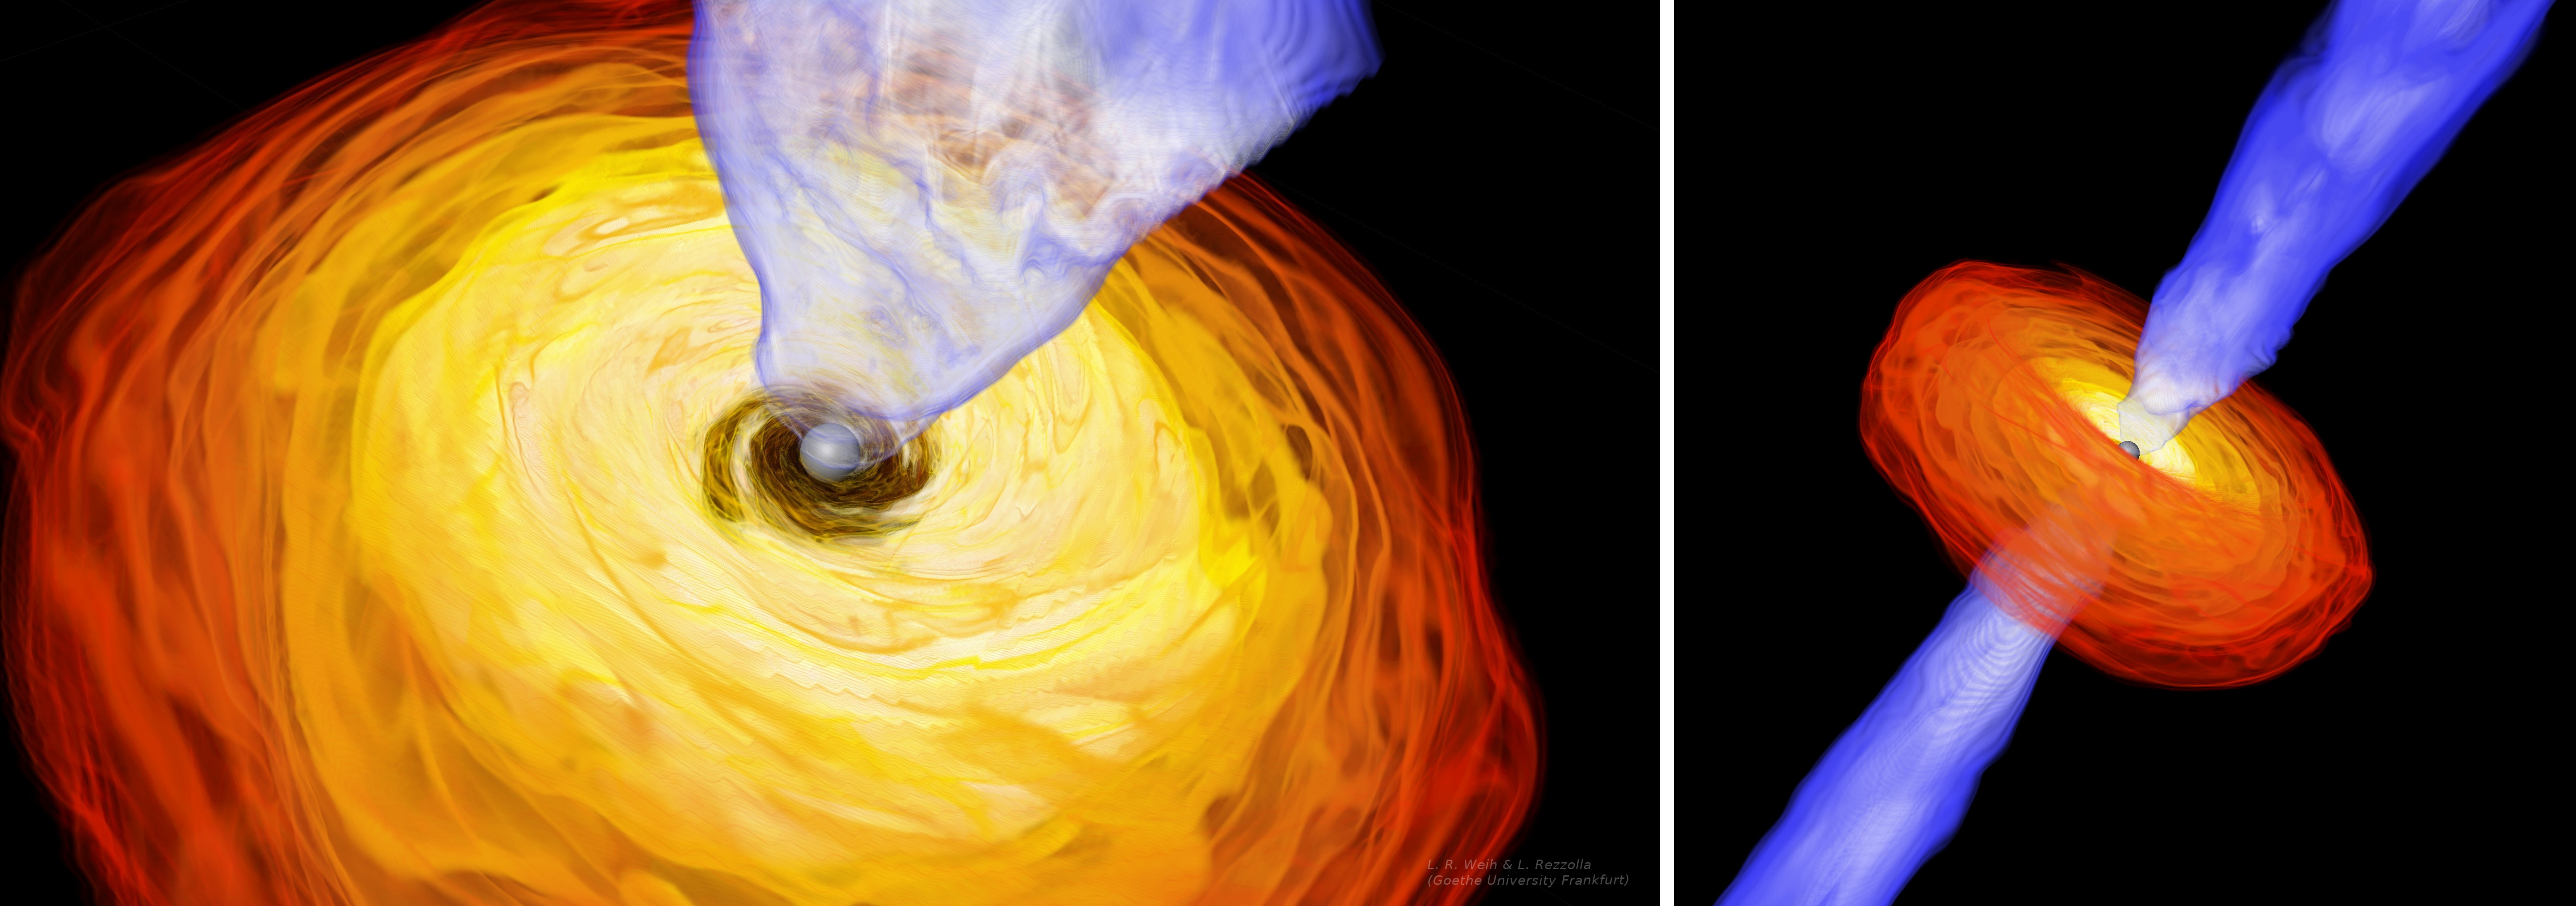
\includegraphics[width=0.88\linewidth,height=0.48\textheight,keepaspectratio]{../figs/pdf/en/fig-07-10.pdf}

% DOCX paragraph 1014
\caption{\emph{Snapshots from a numerical simulation of the dynamics of the plasma
accreting onto a black hole. Note the presence of an accretion disc of matter and of two
relativistic jets. © EHT/L. Weih /LR.}}\label{fig:07-10}
\end{figure}

% DOCX paragraph 1016
Unfortunately, with the exception of the speed of propagation, very little is known
about the composition of the matter inside the jet, although it seems plausible that it
is made up of very light charged particles, such as electron\index{electron}s and
positrons.\textsuperscript{\hyperlink{note:07-08}{8}} Also unknown is what launches the matter inside the
relativistic jets\index{relativistic!jet} and accelerates it to enormous speeds, thus
transferring vast amounts of energy. As you can easily imagine, there is no shortage of
ideas about what is behind the launching and acceleration of these jets, but also no
firm conclusion as yet.\textsuperscript{\hyperlink{note:07-09}{9}}

% DOCX paragraph 1017
Finally, to add a further veil of uncertainty to the many that already envelop
relativistic jets, we do not understand well the processes behind the
collimation\index{relativistic!jet (collimation)}\index{relativistic!jet (stability)} and stability of these jets; namely,
processes that allow them to retain their thin elongated shape over enormous
length-scales without breaking apart or dispersing in the surrounding space. These
processes are so efficient that the jet of M87 remains collimated on a length-scale that
exceeds its section by eight orders of magnitude. To appreciate what this means, let's
consider a relativistic jet as if it were the smoke coming from an ashtray containing a
discarded cigarette with a diameter of about one centimetre. Well, to replicate what we
observe in M87, the cigarette smoke would need to remain collimated, without breaking,
over a length of about a thousand kilometres, more than the distance between London and
Inverness. So, it should now be clear that, whatever its origin, the collimation process
is as effective as it is extreme!

% DOCX paragraph 1018
Let me end this section with a deliberation that I consider very important in the
context of scientific dissemination, especially nowadays when it is so difficult to
distinguish truthful information from misinformation, science and rigour from ignorance
and superficiality.

% DOCX paragraph 1019
It is essential to underline that there is a fundamental difference between the images
created through numerical simulations and those that we often see on the glossy covers
of popular-science magazines or websites dedicated to public outreach. The latter are,
in general, ``artistic impressions\index{black hole!artistic impressions}'', that is, suggestive
representations of how black holes ought to appear in artists' interpretations. Such
images are often the result of a collaboration between experts in computer graphics and
astrophysicists, but, despite the best of intentions, they are not necessarily
consistent with the laws of physics and, most often, constructed simply to please or
excite our imagination.

% DOCX paragraph 1020
By contrast, the images of black holes or jets obtained through numerical simulations,
which may even be interesting from an ``artistic'' viewpoint (see, for instance, Figure
\ref{fig:07-10}), are the result of the solutions to complex equations (examples of these equations
reported in this book are of general-relativistic magnetohydrodynamics around a rotating
black hole). By their very nature, therefore, these images are consistent with the laws
of physics, as they are based on equations that we consider to be faithful
representations of reality near a black hole.

% DOCX paragraph 1021
However, such images do not yet tell us how a supermassive black hole would appear to an
observer. If we want to understand what we would see if we were to observe a
supermassive black hole with radio-sensitive eyes, we need to make an additional effort.

% DOCX paragraph 1024
\section{From A Turbulent Plasma To A Map Of Light}\label{sec:07-map}

% DOCX paragraph 1026
Although physically consistent and possibly graphically appealing, the images resulting
from numerical simulations do not reveal what we might see if we were near a rotating
black hole and our eyes were sensitive to radio waves\index{waves!radio}. These images
tell us how \emph{matter} is distributed and not how and where \emph{light} is produced.
Obviously, if there is no matter, there is no light source either, so there is no
possibility of creating an image. However, the presence of matter is only a necessary
condition; we still need to know how the source of light is distributed and how the
source produces the light. This is because not all of the matter present is a source of
light, and not all of the matter that can produce light does produce the light that we
receive.

% DOCX paragraph 1027
To make this concept slightly more understandable, think of the strings of coloured
lights that we use to decorate Christmas trees. Let's imagine one consisting of a long
sequence of coloured LED lights, where not all the lights are working because the last
celebrations were quite lively, and somehow abundant amounts of sparkling wine managed
to shower the tree~... Let's say that only half of the lights are working, but we do not
know which are failing. We could take our string of lights and decorate our Christmas
tree, noting the exact position of each light as the sequence is distributed on the
tree. At this point, we could turn off the lights in the house and turn on the Christmas
tree lights. As you can imagine, although we know the position of each light, we cannot
yet know what ``image'' of the tree we will receive, that is, what sequence of lights we
will obtain once we turn them on. In particular, we do not know whether a light of a
given colour and position will emit light or not, so we are left with a wide assortment
of possible combinations, all of which are viable, but only one of which will actually
be realised in practice when we turn the decorations on~...

% DOCX paragraph 1028
Well, this is not so different from what happens with our simulations of the plasma
dynamics around a black hole. Our solutions tell us precisely where the matter is and
what its properties are. However, it does not reveal which parts of this matter can emit
light, nor how intense this radiation is. So, as you can imagine, we now have to deal
with an additional complication. Together with understanding what happens to matter
around a black hole, we also need to introduce an \emph{``emission model''}, a model for
the emission of light in the accretion flow. In other words, we need a mathematical
model that allows us to associate the properties of the plasma most important for the
emission of light (the density and temperature of the electron\index{electron!energy distribution}s) with
a physical model expressing how much radiation is emitted in the radio band. Going back
to our Christmas decorations, we need a model that tells us which of the lights in the
string is working, its colour, and the brightness of the light it can emit.

% DOCX paragraph 1029
Finally, as if the whole framework for the emission of radiation was not complicated
enough, we have seen that the light emitted around a black hole can follow very bizarre
trajectories. As a result, we need to ascertain whether the radiation from a region of
the plasma\index{plasma!emission} having the correct conditions to emit such radiation would
actually reach a distant observer. At the same time, we cannot discard a region of the
plasma with only a weak luminosity on the assumption that this may be undetectable. It
is possible that the emission from this region is weak, but it could be intensified by
gravitational lensing\index{gravitational!lensing} and relativistic amplification, thus becoming
visible to a distant observer.

% DOCX paragraph 1030
To recap, I think it is now clear that performing simulations of accreting plasma is
only the first step in obtaining the image of a supermassive black hole. The next
equally challenging and complex step is to predict how the computed distribution of
matter emits light and how this light propagates near the black hole until it reaches
us. To accomplish this requires solving the ``radiation transport\index{radiation transport}''
problem, which amounts to calculating the trajectory of each light ray in the curved
spacetime around the black hole and evaluating the interaction that the light ray will
have with the matter it encounters on its way. Under realistic conditions, light rays
will not propagate in a vacuum\index{vacuum}, and their trajectories will
inevitably intercept (often repeatedly) the accreting matter before reaching us, the
observers. Furthermore, depending on the physical conditions encountered by the light
ray at each point of its path, the interaction with the plasma\index{plasma!emission} can
either decrease the intensity of the light ray (if the matter absorbs the light ray) or
increase it (if additional light emitted by that portion of the plasma is added to the
initial ray). Given the complexity of computing these variations, which will take place
along the trajectory of each light ray for millions of rays, this step in the
theoretical construction of the image can only be accomplished through expensive
simulations performed on parallel supercomputers\index{supercomputers}. And that's exactly
what my research group in Frankfurt has done.

% DOCX paragraph 1031
I am leaving aside the technical details of how the problem of radiation
transport\index{radiation transport} is solved in practice, which are numerous and not
particularly important for this discussion. Instead, in Figure \ref{fig:07-11}, I have
schematically brought together the three most important phases of the process that
ultimately lead to the construction of a \emph{synthetic} (i.e., purely theoretical)
\emph{image}\index{synthetic image} of an accreting supermassive black hole.

% DOCX paragraph 1033
\begin{figure}[htbp]
\centering
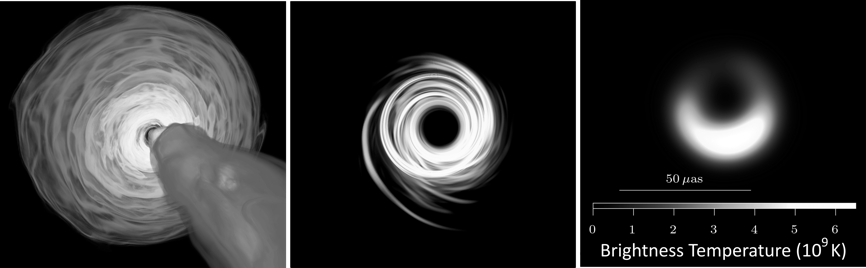
\includegraphics[width=0.88\linewidth,height=0.48\textheight,keepaspectratio]{../figs/source/en/fig-07-11.png}

% DOCX paragraph 1035
\caption{\emph{The three phases of making a synthetic image. © L. Weih/C. Fromm/Z.
Younsi/LR.}}\label{fig:07-11}
\end{figure}

% DOCX paragraph 1037
In particular, the left panel shows the result of a simulation of plasma dynamics,
revealing the distribution of the plasma in the accretion disc and the magnetic fields
in the jet (see also Figure \ref{fig:07-10}). The panel in the middle, on the other hand, shows the
emission in the radio band (particularly at the frequency of 230 GHz) as calculated
based on the distributions shown in the left panel. In other words, it illustrates how
the matter placed in the left panel would appear if we had eyes sensitive to radiation
in the radio band. Finally, since the central panel in Figure \ref{fig:07-11} shows an \emph{ideal}
synthetic image\index{synthetic image}, that is, relative to a perfect instrument without
any noise\index{noise}, the panel on the right shows how the emission would really
look if recorded through a network of radio-telescopes connected with the VLBI technique
and, therefore, with a resolution that is high but finite. All the images in the three
panels are made with a viewing angle reflecting that at which we think we are observing
M87*\index{M87*}.

% DOCX paragraph 1038
Overall, Figure \ref{fig:07-11} offers us a cue for several considerations. First, when moving from
the left panel to the middle panel, we can readily appreciate how not all of the
accreting matter contributes to the emission of radiation in the radio band (for
instance, the jet contributes little in this specific image). Furthermore, the maximum
intensity of the emission is not always linked to areas with maximum density, even
though, in general, a good portion of the emission comes from the inner parts of the
disc, which are also those where the density is highest.

% DOCX paragraph 1039
Second, the image in the middle panel represents the combination of all the light
contributions produced in the vicinity of the black hole and which, once deflected and
amplified, can reach a distant observer. Hence, although the light we see in the picture
is emitted largely by the disc, it is also produced by the jet moving towards us (i.e.,
the ``approaching'' jet) \index{relativistic!jet (approaching)}, and even by the jet moving away from us
(i.e., the ``receding'' jet\index{relativistic!jet (receding)}). This is possible because, as we have
seen, light emitted in the opposite direction to our line of view can still be deflected
and reach us if the accreting matter in this radio band is ``optically thin'',
essentially transparent. However, if it were ``optically thick'', the light from the
receding jet would be absorbed, and the jet would be invisible.

% DOCX paragraph 1040
Finally, the panel on the right reminds us that the resolution it is possible to obtain
with current technology, although the highest ever, is still far from what we would like
and from what would allow us to derive extensive information from the image of a black
hole. However, Rome was not built in a day, and the process of producing the image of a
black hole does not end with the results obtained by the EHT in 2019. On the contrary,
the image presented in Figure \ref{fig:07-01} must be considered as the beginning of a process that
will take decades to reach a complete development.

% DOCX paragraph 1041
Before concluding this section, let's return for a moment to the analogy of the matter
accreted by a black hole and the flow of water measured at a waterfall. We have seen
that the motion of matter around the black hole is turbulent in nature and therefore
fundamentally irregular, even if it has precise statistical properties, such as average
values and fluctuations of almost constant amplitude. If the motion of matter is
turbulent and fluctuating, then so too must be the emission of light from that matter.
The implication of this is as trivial as it is important. There cannot be a
\emph{single} and \emph{static} image of M87*\index{M87*}; the image must
necessarily be dynamic and fluctuating to represent the state of matter around the black
hole over a certain time.

% DOCX paragraph 1042
When you come to think of it, this conclusion isn't surprising at all. Imagine taking a
series of photos of a mountain at different times, similar to making a video with the
time-lapse technique. The various images we take will be very similar, but none will be
identical to the previous one, perhaps because a cloud has moved or the lighting
conditions have changed slightly. What happens to our simulations, and therefore to our
radio observations, is not very different when we try to produce an image of
M87*\index{M87*}. The distribution of matter will change continuously, and so
will the radio emission. So, the image we are trying to produce will inevitably be
subject to variability\index{variability}, much like taking a picture of a very active
toddler who pays no heed to our appeals to stay still. In such a case, we all know that
the only way to get images that are not shaky is to use exposure times that are shorter
than the typical timescale over which the subject changes. In essence, we need to shoot
faster than they move!

% DOCX paragraph 1043
So, you may be wondering: ``What is the timescale of variation of the emission in
M87*\index{M87*}?''. Although it reflects very complex dynamics, the answer to
this question is fortunately very simple: the timescale depends on the black hole mass.
To be precise, it can be associated with the time roughly needed to travel a circular
orbit\index{orbit} around the black hole. In the simplest case of a nonrotating
black hole and an orbit placed near the light-ring, this timescale is given by
\(\tau\sim(3GM/c^{3})\), where the estimate takes into account that it is sufficient to
consider only a portion of the orbit and that the latter can also be at radii smaller
than the light-ring.

% DOCX paragraph 1044
If we calculate this timescale for the estimated mass of M87*\index{M87*}, that
is, 6.5 billion solar masses, we would conclude that the variability\index{variability}
timescale is of the order of 24 hours. Therefore, although the source of radiation
around M87* is intrinsically fluctuating, it will effectively appear as nearly static
provided we use exposure times of less than one day. Since the EHT observations took
place over a time window of about 8 to10 hours (the timescale over which M87* becomes
visible to the first telescope in France and then disappears for the last telescope in
Hawaii), the VLBI images are essentially static. If a variable is present, this should
be minor and only appear when comparing across different days --- which is exactly what
the observations have shown!

% DOCX paragraph 1045
A quasi-stationarity in the emission is unfortunately not present in the case of Sgr A*,
whose mass is almost a thousand times smaller than that of M87*\index{M87*} and
whose expected variability\index{variability} is, therefore, of the order of only a few
minutes. Under these conditions, the VLBI observations would somewhat resemble a short
and incomplete film, which is, of course, much more complex to analyse and interpret.
The EHT is currently involved in the final analysis of the VLBI observations of Sgr A*,
whose image should be published before the summer of 2022.

% DOCX paragraph 1046
I want to close this section with a question some might ask: ``Should we take into
account changes in the mass of the black hole due to the accretion of matter during the
observations?''.

% DOCX paragraph 1047
This question would be very interesting, and I can provide a simple and categoric
answer: no, we need not worry. The timescales for the variation of the mass of a
supermassive black hole are, in fact, enormous compared to those over which the
observations are carried out. To grasp what this means in practice, let me remind you
that the observations of M87*\index{M87*} have allowed us to estimate that its
mass increases by one single solar mass over four hundred years of accretion.
Considering that the total mass of M87* is billions of solar masses, then over ten
million years, it will increase its mass at most by one part in a million. After all,
this is not so different from when we take our time-lapse photos of the mountain. Also,
in this case, we know the mountain will change while we take a series of pictures;
slowly but inexorably crumbling due to erosion so, in about ten million years, a large
part of it will end up in the sea. However, because we know these changes are so minute,
we simply don't think about them when taking our time-lapse video of the beautiful
mountain~\ldots{}

% DOCX paragraph 1053
\section{The Images Of M87*}\label{sec:07-images}\index{M87*}

% DOCX paragraph 1055
In the previous pages, I have emphasised that carrying out
plasma-dynamics\index{plasma} simulations is conceptually not dissimilar to what
meteorologists do with their weather forecasts. However, there is a significant
difference: while weather predictions refer to a relatively narrow window in the future,
ranging from a few hours to a few days, after which they lose reliability, our
simulations cover much longer timescales of the order of about a decade.

% DOCX paragraph 1056
This point may be quite surprising for some of you and begs the obvious question: ``Why
on earth do the simulations cover a period of ten years when the observations last less
than a day?''. The simple answer is that we run our simulations on such a long timescale
in order to build reliable statistics for the possible accretion states of the black
hole. In this way, following the VLBI observations and reconstruction of an image of the
black hole, we can compare this image to an extensive ``library'' of synthetic
images\index{synthetic image!library} of an accreting supermassive black hole. For this reason, and
to use a previous analogy, we do not take a single photo of our mountain but take
several photos every day for ten years. The hope is that if we ever find ourselves with
a blurred photo that could be of a mountain, our rich catalogue of images of mountains
under various conditions will allow us to understand whether it is a mountain and
possibly deduce its properties.

% DOCX paragraph 1057
Following this logic, scientists of the EHT, and in particular the research group in
Frankfurt, have engaged in the most extensive and systematic campaign of numerical
simulations of accreting black holes ever attempted before. The aim was to construct the
broadest and most complete description of the physical conditions encountered by a
plasma when accreting onto a black hole. Using complex and sophisticated numerical codes
and exploiting a multitude of parallel supercomputers\index{supercomputers}, a large number
of simulations at very high angular resolution\index{angular resolution} were performed,
covering all of the most important scenarios in which a supermassive black hole can
accrete matter.

% DOCX paragraph 1058
In particular, we have carried out simulations by varying one or more of the following
parameters:

% DOCX paragraph 1059
\begin{itemize}
\item \emph{The spin of the black hole}. Considering both nonrotating and very rapidly
rotating black holes.

% DOCX paragraph 1060
\item \emph{The direction of rotation of the plasma in respect to the black hole}. Studying
plasma that is either corotating or counter-rotating with the black hole.

% DOCX paragraph 1061
\item \emph{The strength of the magnetic field.} Exploring two different types of accretion
discs that differ in the accretion rate they can produce and which can either be small
or large.
\end{itemize}

% DOCX paragraph 1062
You may have noticed I have not mentioned the mass of the black hole as a parameter that
could vary; this is because all of the black holes considered had exactly the same mass.
This was possible because, although the mass of the black hole plays a very important
role, it can easily be factored out of the problem. All of the quantities computed in
the simulations, in fact, can be properly rescaled, so the same simulation can be used
to describe the accretion onto a black hole of one solar mass or one billion solar
masses.

% DOCX paragraph 1063
It is not helpful at this point to discuss the many simulations performed, each of which
has allowed us to produce hundreds of distinct synthetic images\index{synthetic image}.
Suffice it to say that the simulations covered a large variety of scenarios, each
different from the others. In some simulations, the accretion disc is very bright while,
in others, it has a very weak emission. In some cases, the disc terminates very near the
horizon (generally, this happens for highly spinning black holes with the plasma in
corotation). In others, it terminates very far away (this instead happens for black
holes that are highly spinning but with the plasma in counter-rotation).

% DOCX paragraph 1064
Finally, to further enlarge the range of possible synthetic images, each simulation was
accompanied by a variety of emission models that specified the energetic properties of
the electron\index{electron!emission model}s responsible for the radiation in the radio band. As a
result, using the same numerical simulation produced a wide variety of additional
realisations of the synthetic images, generating a new sequence for each of the emission
models employed.

% DOCX paragraph 1065
In its effort to build a theoretical interpretation of the observations and extract as
much information as possible, it comes as no surprise that, in just over six months, the
EHT has produced as many as \emph{60,000 synthetic images}\index{synthetic image}. These
images cover the majority of possible configurations in which an accreting black hole
could appear. This huge library of synthetic images is even more impressive when you
bear in mind that we didn't know how M87*\index{M87*} was oriented concerning our
line of sight. Indeed, this is one piece of information we wanted to learn from
observations. Hence, each synthetic image alone can generate hundreds of other images
simply by changing the two angles under which the image can be rotated.

% DOCX paragraph 1066
From a conceptual point of view, each of these 60,000 images represents a plausible and
physically consistent realisation of how an accreting supermassive black hole might look
when viewed with a network of VLBI-connected radio-telescopes. However, it is also
possible that none of these 60,000 \emph{synthetic}\index{synthetic image} images
corresponds to any one of the four \emph{observed} images reconstructed by the EHT based
on data collected on April 5, 6, 10, and 11, 2017, and on which I report below.

% DOCX paragraph 1068
\begin{figure}[htbp]
\centering
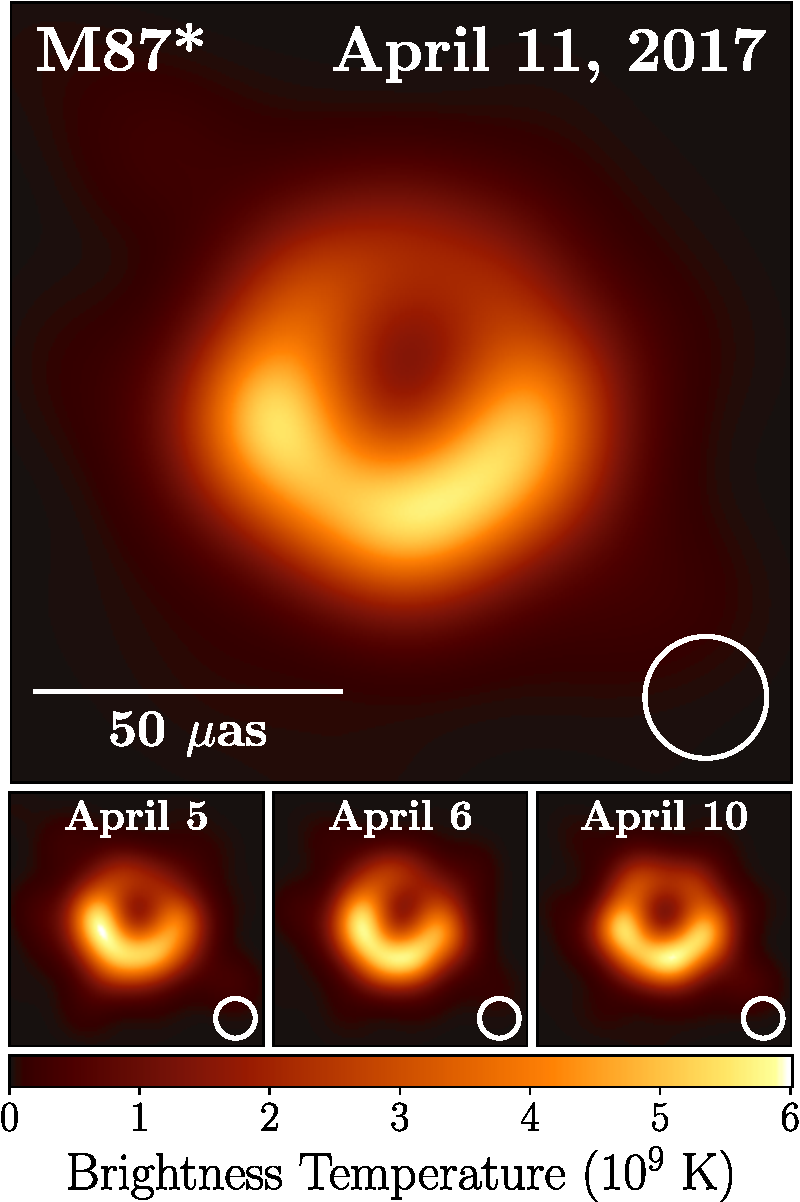
\includegraphics[width=0.88\linewidth,height=0.48\textheight,keepaspectratio]{../figs/pdf/en/fig-07-12.pdf}

% DOCX paragraph 1070
\caption{\emph{Four different images of M87*}\index{M87*} \emph{taken on
different days in April 2017 by the EHT Collaboration at a radio frequency of 230 GHz. ©
The EHT Collaboration.}}\label{fig:07-12}
\end{figure}

% DOCX paragraph 1072
Clearly shown in Figure \ref{fig:07-12}, and as expected, these observed images show some variation
from one day to another but also reveal an overall ``robustness'' of the basic
properties of the images.

% DOCX paragraph 1075
\section{Like A Needle In A Haystack}\label{sec:07-needle}

% DOCX paragraph 1077
Allow me to give you a recap of the long sequence of events and arguments made so far.
In April 2017, after months of preparations, the EHT performed VLBI observations of
M87*\index{M87*} and, after more than one year of work on the data, it was able
to reconstruct four observed images. Meanwhile, between the end of 2018 and the
beginning of 2019, the EHT ran a massive campaign of theoretical simulations, trying to
predict how a supermassive black hole surrounded by accreting plasma\index{plasma!accreting}
should look, thus producing 60,000 synthetic images. I have not yet described the final
step in our analysis and the missing piece in the big puzzle that has led to the first
photo of a black hole. This step is necessary to find which of the 60,000 synthetic
images correspond to the four observed images so that the EHT could finally learn what
the observations were all about. Although this may seem very simple to take from a
logical point of view, it is much like looking for the notorious needle in a
haystack~\ldots{} Fortunately, we could use computers to overcome this final challenge.

% DOCX paragraph 1078
There are sophisticated mathematical algorithms that make it possible to solve problems
of this type (which are very complex and characterised by multiple possible parameters)
by exploiting the computational power of large supercomputers\index{supercomputers}. Here,
we can ignore the technical details of algorithms\index{algorithm!Markov chain} with appealing
names, like ``Markov chain Monte Carlo'' or ``genetic\index{algorithm!genetic}''. I would just
mention that these algorithms can find an optimal (or quasi-optimal) solution to
problems using large amounts of data that depend on many parameters. Once applied to the
data and a ``best-fit'' is found for the data and the model, these algorithms quantify
the probability that a given parameter is contained in a certain interval. In this way,
it was possible to compare the four observed images with the synthetic ones and
determine the probabilities that a certain parameter, for example, the mass of the black
hole or its spin, would fall within a certain interval.

% DOCX paragraph 1079
To better understand how this matching process works in practice, let's perform another
gedanken experiment. Just imagine you are in a stadium hosting 60,000 spectators who are
anxiously waiting for an important game to start. On entering the stadium, you catch a
glimpse of someone that looks like a good friend of yours whom you lost in the bustling
crowd at the entrance. Hence, you are not sure the person you have seen is your friend
and, if it is, whether or not they are now in the stadium. Luckily, you happen to have a
recent but very blurred photo of your friend with you. Security at the stadium is based
on CCTV cameras that capture pictures of each person as they enter the stadium. So, you
approach the kind manager of the surveillance system and ask him to compare your blurred
photo with the high-resolution mugshots taken at the entrance by the fixed cameras. The
comparison process the surveillance system performs will use Markov chain Monte Carlo or
genetic algorithms to find the best match for the images taken at the entrance and that
of your friend. In practice, facial recognition techniques will be used, which decompose
a human face into main features (for example, the distance between the eyes, the
position of the nose in respect to the eyes, the size of the mouth, etc.). Essentially,
each mugshot is decomposed into a series of parameters (basically \emph{N} numbers),
with one parameter for each facial aspect. The algorithms then compare the sequence of
\emph{N} numbers corresponding to your blurred photo with the \emph{N} numbers for each
of the 60,000 images in the library of mugshots. The ``intelligent'' part of the
algorithm lies in looking for the best match without accessing the entire library, but
instead ``moving'' within the space of \emph{N} sequences in an efficient manner,
concentrating only on those sequences for which there is already a good match. In this
way, the search is simpler and, above all, faster.

% DOCX paragraph 1080
Figure \ref{fig:07-13} offers a schematic representation of this process. The top left image is the
blurred photo of your friend (which, at least from a logical point of view, is similar
to Figure \ref{fig:07-01}), and the image in the top right is a comparison from the library of
mugshots (consisting of 54,200 images to be precise).\textsuperscript{\hyperlink{note:07-10}{10}} The two rows
below show ten photos from the library selected by the algorithms as those closest to
the reference image. From a mathematical viewpoint, the images in the rows below are
those that received the highest ``scores'' in the comparison of the parameters
associated with your friend's face.

% DOCX paragraph 1081
The process of image comparison shown in Figure \ref{fig:07-13} (conceptually very similar to what
was done for M87*\index{M87*}) teaches us some important lessons. First, it
reveals that the mathematical operation of projection of the reference image into the
space represented by the library of images of spectators in the stadium is not unique;
that is, the projection is degenerate. In terms that are perhaps easier to understand,
the comparison process reveals that, in general, there are multiple candidates. In our
case, there are at least ten (there could be more or less depending on the tolerance of
our algorithm) who, essentially with the same score, meet all of the criteria we imposed
to find an image that is ``sufficiently similar'' to that of your friend. No surprise
here; as in the case of the wall clock, as long as the amount of information available
to us is limited and restricted to observations, a multiplicity of possible answers is
almost inevitable.

% DOCX paragraph 1082
\begin{figure}[htbp]
\centering
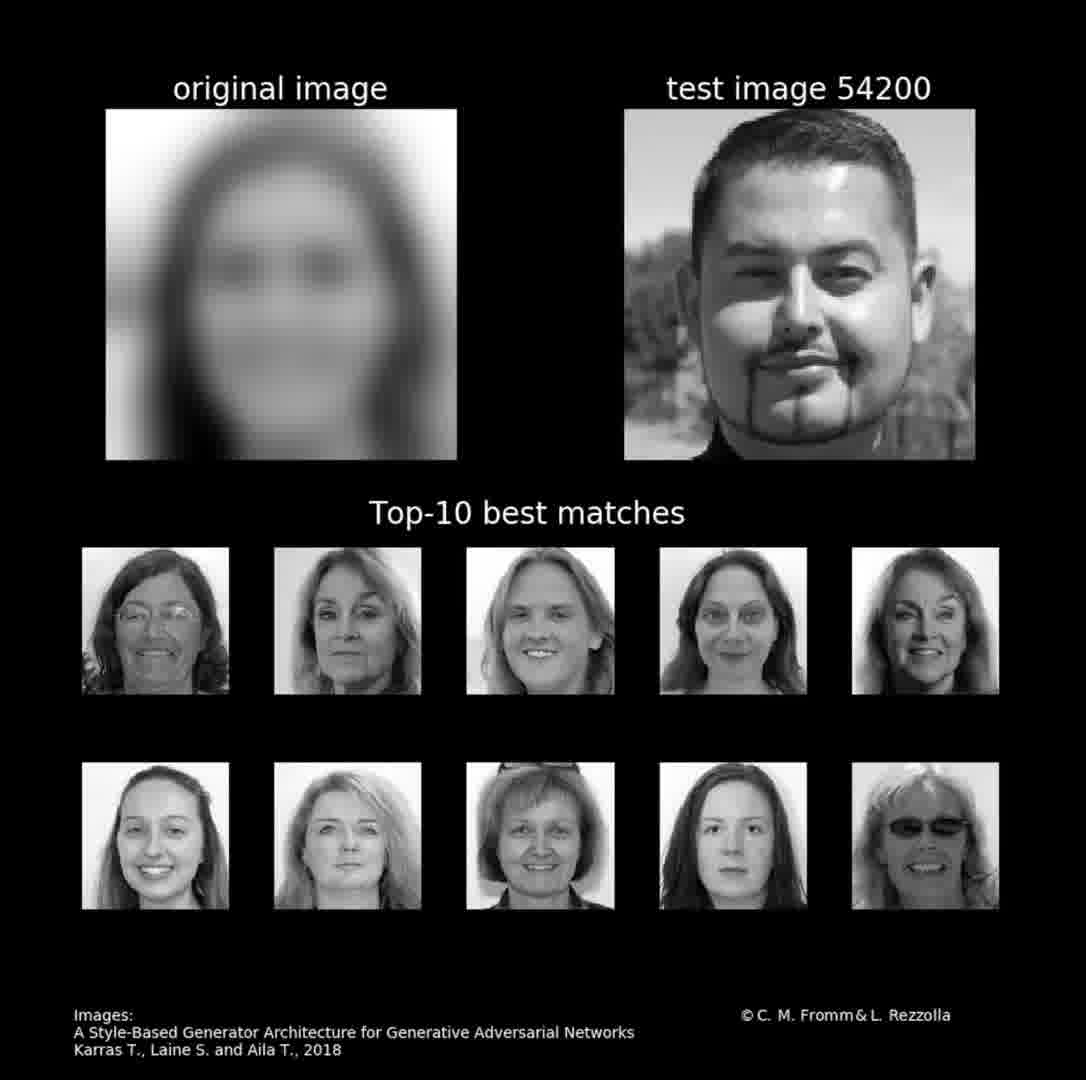
\includegraphics[width=0.88\linewidth,height=0.48\textheight,keepaspectratio]{../figs/source/en/fig-07-13.jpg}

% DOCX paragraph 1084
\caption{\emph{Image comparison process. © C. Fromm/LR. Images: T. Karras, S. Laine, T.
Aila.}}\label{fig:07-13}
\end{figure}

% DOCX paragraph 1086
Second, while there are good matches, it appears that your friend is not at the stadium
since none of the best images seems to correspond to the reference image, even though
some are quite close. Please note, I wrote ``seems'' because these face-recognition
algorithms only measure the probability of a certain match, and this probability is
never 100\% unless we are dealing with ``perfect'' images, that is, without noise or, if
you like, perfectly sharp and at very high resolution. Also, in the comparison between
the observed images of M87*\index{M87*} and the synthetic ones, the result of the
match is measured in terms of probabilities. Notwithstanding that, we have done our best
to create a synthetic image\index{synthetic image} as close as possible to reality; the
latter is always more complex than we can represent with our simulations. Therefore, it
is perfectly plausible and scientifically acceptable that none of the hundreds of
thousands of images produced synthetically corresponds ``exactly'' to the one observed.

% DOCX paragraph 1087
The properties of the ten best-matched images in the lower rows provide the third and
last lesson. The selection given by the algorithms reveals that your friend belongs to a
particular class of human beings: a female with long hair. This is because all of the
subjects in the best-matched images are women. Although there were also men in the
stadium with long hair, the face recognition algorithm didn't pick any of them out,
revealing that your friend has long hair and also is a woman.

% DOCX paragraph 1088
Of course, you might argue that this result is trivial: you already know that your
friend is a woman and that she has long hair. However, regarding the image of
M87*\index{M87*}, we did not know what class of object the image referred to.
Hence, just by studying the properties of the best matches, we could learn a lot about
the image, even if we did not find a perfect match!

% DOCX paragraph 1089
Let's return now to what we have actually done with the EHT and M87*\index{M87*}
and set aside friends and events in the stadium. Figure \ref{fig:07-14} illustrates this by showing
the excellent comparison between the image of M87* observed on April 11, 2017 (left
panel) and a synthetic image\index{synthetic image} appropriately blurred to take into
account the experimental noise\index{noise} (right panel).

% DOCX paragraph 1090
\begin{figure}[htbp]
\centering
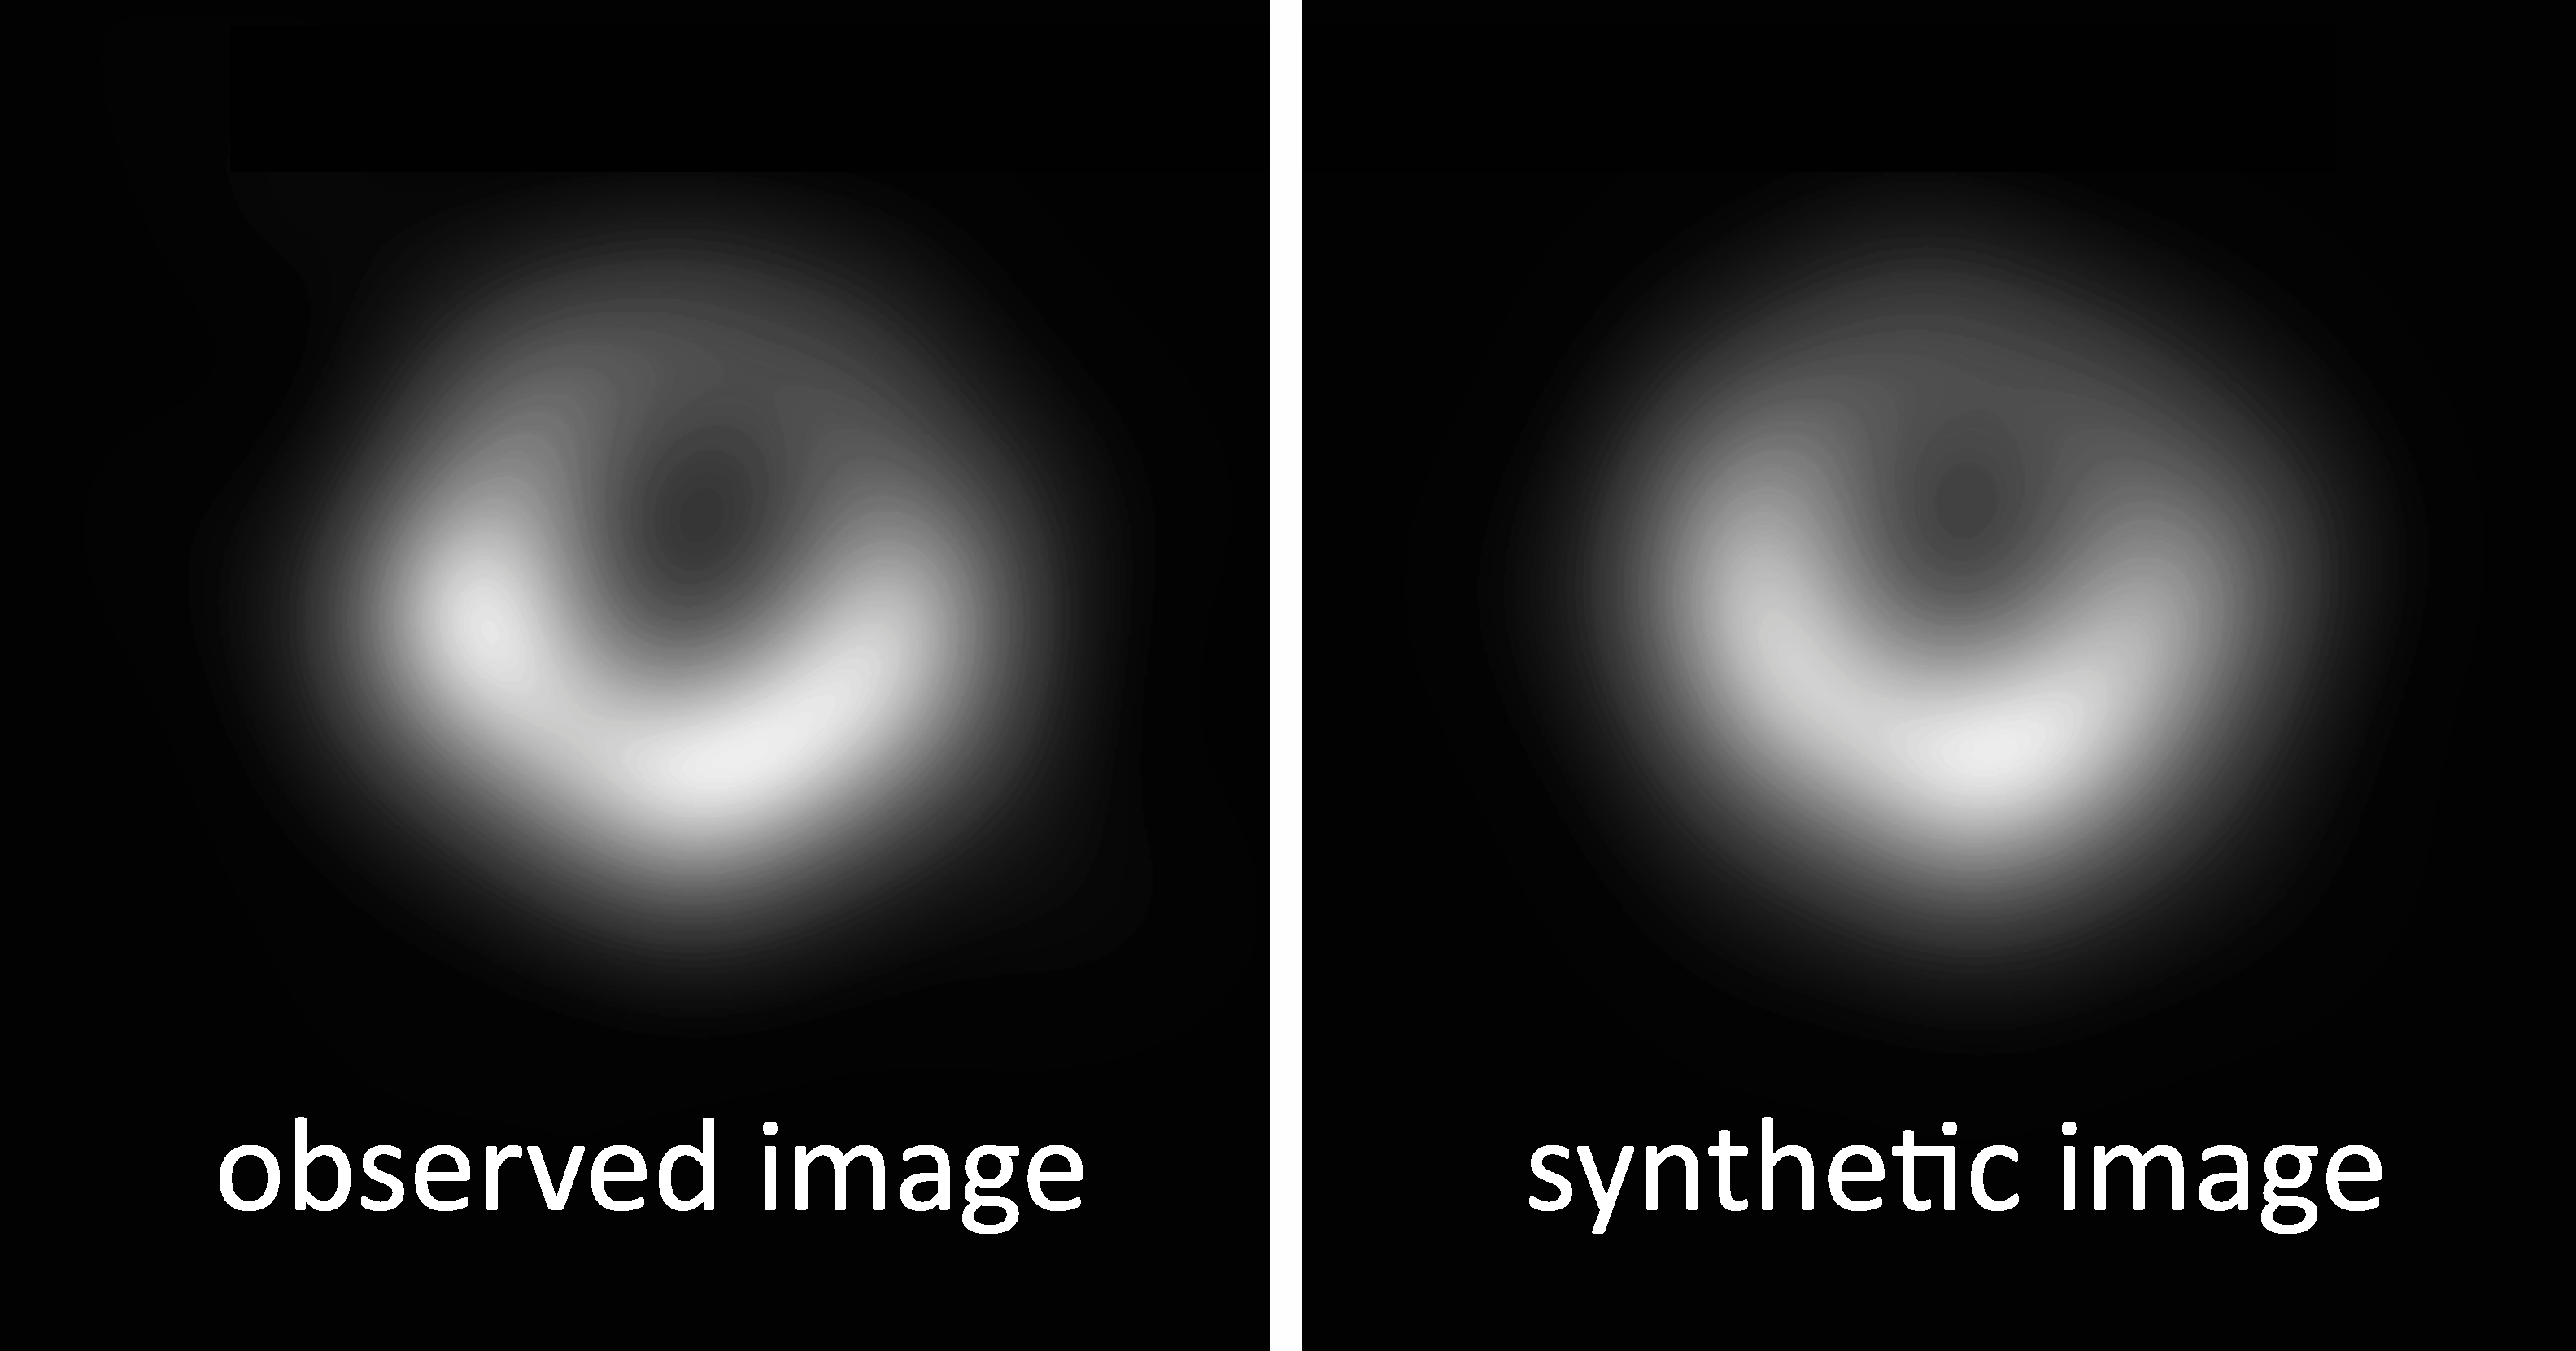
\includegraphics[width=0.88\linewidth,height=0.48\textheight,keepaspectratio]{../figs/pdf/en/fig-07-14.pdf}

% DOCX paragraph 1092
\caption{\emph{Example of the excellent match between an observed image of
M87*}\index{M87*} \emph{and a suitably deteriorated synthetic image. © The EHT
Collaboration/C. Fromm/LR.}}\label{fig:07-14}
\end{figure}

% DOCX paragraph 1094
I think it is clear that the similarity between the two is impressive. In fact, the
score that the algorithms have assigned to the image on the right is among the highest
found among the hundreds of thousands of synthetic images produced.

% DOCX paragraph 1095
The image on the right is a fully theoretical prediction. It was produced through
simulations of plasma dynamics and by employing a precise model for the emission of the
radiation. Hence, we know every feature of the object behind the image on the right: the
mass and spin of the black hole, the inclination with respect to the observer, the
temperature and energy distribution of the electrons, etc. Logically, we could then
believe that we also know everything about the image on the left. However, this logic,
albeit simple, is unfortunately flawed! The simple reason is that, although the image on
the right offers a very close theoretical representation to the observed reality, it is
unfortunately not unique. Just as for the women shown in the ten small panels in Figure
\ref{fig:07-13}, in fact, there are also degeneracies in the case of M87*\index{M87*} that
cannot be removed and that are the direct consequence of the finite (basically low)
resolution at which the observed image has been constructed.

% DOCX paragraph 1096
The most important consequence of this degeneracy\index{degeneracy!intepretation} is that we have
found a number of synthetic images\index{synthetic image} that match equally well-observed
images but refer to very different models of black holes, for instance, to a nonrotating
black hole or to a black hole that is maximally rotating. This result, which at first
glance might seem impossible, is instead perfectly plausible; it is the consequence of
using different models for the emission of radiation. It is thus possible that two
different emission models applied to two different accretion models conjure up almost
identical low-resolution images. In other words, the differences in spin and emission
can combine in such a way as to produce two images that our algorithms recognise as
being very similar.

% DOCX paragraph 1097
This result is not too surprising given the novelty and quality of the first
observations of M87*\index{M87*} and is both ``bad'' and ``good''. It is ``bad''
in the sense that it reveals that, with our observations, we are unable to appreciate
the differences introduced by the spin of the black hole and its orientation (in other
words, our observations are ``insensitive to spin''). Consequently, we cannot really
measure the spin of M87* and, indeed, the EHT publications in 2019 do not report any
estimate for the spin of M87*. At the same time, this degeneracy\index{degeneracy!intepretation} is
``good'' because it lets us conclude with great confidence that Figure \ref{fig:07-01} does indeed
show a supermassive black hole. In fact, all of the synthetic images\index{synthetic image}
that best match the observations always correspond to a simulation of an accreting black
hole and, under all conditions, yield an image as in Figure \ref{fig:07-01}, regardless of the value
of the spin.

% DOCX paragraph 1098
Exactly this happened in our gedanken experiment at the stadium; the face recognition
algorithms didn't inform us with any certainty about the presence of your friend.
However, they did inform us, with very high confidence, that your friend belongs to the
class of human beings that are women with long hair and not men with long hair.
Similarly, and notwithstanding the degeneracy\index{degeneracy!intepretation} between theory and
observations, we can conclude that the image of M87*\index{M87*} most likely
belongs to the class of compact objects that are black holes, for which it has all the
basic features. And this is indeed a revolutionary result!

% DOCX paragraph 1099
I want to conclude this section with two optimistic considerations. The first is that I
didn't really tell you the whole story when I said we are wandering in the dark
concerning the spin of M87*\index{M87*}. Although we are insensitive to spin if
we limit ourselves uniquely to the EHT images, we have other cards up our sleeves. We
can also consider the observations made in the past by other scientists about the
central object in M87 and this would immediately shed some light on its spin. In
particular, we could use the power emitted by the relativistic jet\index{relativistic!jet} of
M87*, which can be measured with good precision given the huge dimensions of the jet. In
this way, we can rule out that M87* is a nonrotating black hole. This is because all of
our numerical simulations show that Schwarzschild-type black holes do produce jets, but
these are energetically ``too weak'' to explain the jet power measured by the
observations. In essence, with the help of the observations made by other astronomers,
we can conclude with reasonable certainty that M87* must be a rotating black hole, even
if we do not yet know its rotation rate or its direction of rotation.

% DOCX paragraph 1100
The second optimistic consideration is that, as explained in many of the examples I have
given, the degeneracy\index{degeneracy!intepretation} between theory and observation is not destined
to last forever. The images obtained are simply the \emph{first} of
M87*\index{M87*}, and we will be able to produce more images with ever-increasing
precision in the future. Unlike the observations of black holes made through
gravitational waves\index{gravitational waves} (which we will discuss in the next chapter) that
can be carried out only once, we will continue for many decades to take photos of the
remarkable black hole, M87*. These new observations will be more and more accurate and
detailed, not only because they will be made at ever shorter radio wavelengths (let's
not forget what Equation \eqref{eq:07-01} taught us) but also because they will be made by an
increasingly large number of radio-telescopes. Finally, when imaging a future that is
perhaps not too distant, these radio-telescopes will be mounted on satellites and then
connected with the VLBI technique, thus creating baselines of tens of thousands of
kilometres between them, that is, many times the diameter of the Earth.

% DOCX paragraph 1101
In short, the inevitable veil of uncertainty that, for now, surrounds the value of the
spin of M87*\index{M87*} will not remain there for long; we will soon find out!

% DOCX paragraph 1104
\section{Are We Really Sure?}\label{sec:07-sure}

% DOCX paragraph 1106
We have seen that the observations made by the EHT are in agreement with the predictions
of the theory, based on models of accretion onto and emission from black holes. It
follows that the very concept of black holes as expressed by the theory of general
relativity\index{general relativity} is perfectly compatible with the observations.

% DOCX paragraph 1107
Nevertheless, on several occasions, we have paused to reflect that astrophysics, as an
observational science\index{observational!science}\index{science!observational }, must live with the
inevitable possibility of a degeneracy\index{degeneracy!intepretation} between the observations and
the models capable of explaining them. We have also seen that the black-hole solution is
not the only one, even though it represents the most natural and simple explanation to
the phenomenology observed in compact astrophysical objects. Alternative interpretations
involve very compact objects with or without a surface and not having an event
horizon\index{event horizon}. Finally, we have seen how Einstein's theory of general
relativity, whose predictions have always proved correct, does not represent the only
theory of gravity capable of explaining the observations.

% DOCX paragraph 1108
Based on these considerations, you could take one of two stances. A more conservative
stance would assume the only correct interpretation of the EHT observations to be the
simplest and most natural and would involve the concept of black holes in general
relativity\index{general relativity}. In this case, there would be no need for you to read any
further, and you could immediately skip to the next chapter. The second position, more
open and less conservative, is to be aware of an important lesson history has taught us
so far: what appears exotic and abstruse today can become plausible and acceptable
tomorrow. If you feel more inclined towards the second attitude, then you should
continue reading because I will try and address a question that is as simple as it is
fundamental: ``Are we sure that what was imaged by the EHT is a black hole?''.

% DOCX paragraph 1109
Personally and notwithstanding that I have devoted my entire career to studying the
consequences of general relativity (and I firmly believe that this theory, however
incomplete, offers the correct interpretation of gravity), I am definitely among those
with a more open-minded attitude. This is why, together with my collaborators, I
conducted a series of studies aimed at answering the question above. Obviously, I cannot
go into the details of such research here, the technical and mathematical aspects of
which are a poor fit for a popular-science book. However, I can share the most important
conclusions, and I will do this in the remainder of this chapter.

% DOCX paragraph 1110
In essence, the name of the game that my collaborators and I have decided to play is to
extend to other compact objects, either in Einstein's theory or other theories, the
analysis carried out so far on accreting black holes in Einstein's theory. And hence, to
determine to what extent it is possible to distinguish such objects based on the
observations. For this purpose, we carried out the same plasma dynamics simulations we
discussed in the cases of Schwarzschild and Kerr black holes. We also used the same
models of radiation emission with the final goal of obtaining synthetic images of these
``exotic\index{exotic!compact object}'' compact objects. Finally, we used the same information
about the properties of radio-telescopes and their resolution to obtain realistic radio
images.

% DOCX paragraph 1111
In our comparisons so far, we have considered two classes of compact objects. The first
is a \emph{``dilaton}\index{black hole!dilaton} \emph{black hole''} and can be seen as a
generic representative of a class of compact objects that can be an alternative to
Einstein's black holes with an event horizon. Instead, the second class is represented
by a so-called \emph{``boson star}\index{boson star}\emph{''}\index{exotic!compact object (boson star)}, which
does not have an event horizon\index{event horizon}, but has a
compactness\index{compactness!boson star} comparable to black holes. For those who may be
wondering, a dilaton black hole emerges as a solution in the Einstein-Maxwell
dilaton-axion\index{alternative theories (gravity)!dilaton-axion} theory of gravity. This theory couples the
Einstein-Maxwell equations to the dilaton scalar field and the axion
vector\index{vector} fields. In essence, the presence of these two additional
fields breaks the assumption of vacuum\index{vacuum} being needed to obtain a
black-hole solution in general relativity and provides the black hole with additional
properties (``hair\index{black hole!hair}s''). The existence of these two fields is entirely
speculative at this point. A boson star is instead a self-gravitating cloud of a scalar
field (again of underdetermined nature and origin) with a core that can be very compact,
effectively appearing as a black hole in terms of gravitational effects. Our choice of a
dilaton black hole as a representative case for an alternative theory was motivated by
such a solution being physically very distinct from general relativity, as it requires
the presence of an additional scalar field (i.e., the dilaton field), absent in
Einstein's theory. Similarly, the choice of a boson star is linked to this type of
object being discussed often in astrophysics as a possible candidate for dark
matter\index{dark matter}, and because it should have a behaviour very similar to that
of a wormhole, another popular exotic\index{exotic!compact object} compact object we have
encountered.

% DOCX paragraph 1112
Skipping all the details related to these studies, which you can be sure are numerous
and can be found in the corresponding papers\textsuperscript{\hyperlink{note:07-11}{11}}, I have reported in
Figure \ref{fig:07-15} the final comprehensive result of this research. In particular, the figure
shows synthetic images\index{synthetic image}, at a frequency of 230 GHz, of the three
compact objects when they are set to have the same mass and are subject to the same
accretion processes via a geometrically thick disc. The left panel refers to a rotating
black hole in Einstein's theory (i.e., a Kerr black hole\index{black hole!Kerr} with spin
\emph{a=0.6}). In contrast, the centre panel shows a dilaton\index{black hole!dilaton} black
hole with a dilaton parameter \emph{``b''}, such that it has an innermost stable
circular orbit\index{orbit!innermost stable circular} equal to that of the Kerr black
hole\index{black hole!Kerr} (i.e., \emph{b=0.5}). Finally, the panel on the right refers to
a boson star\index{boson star} having a compactness\index{compactness!boson star} of
\emph{M/R≃0.1,} close enough to that of a black hole.

% DOCX paragraph 1114
\begin{figure}[htbp]
\centering
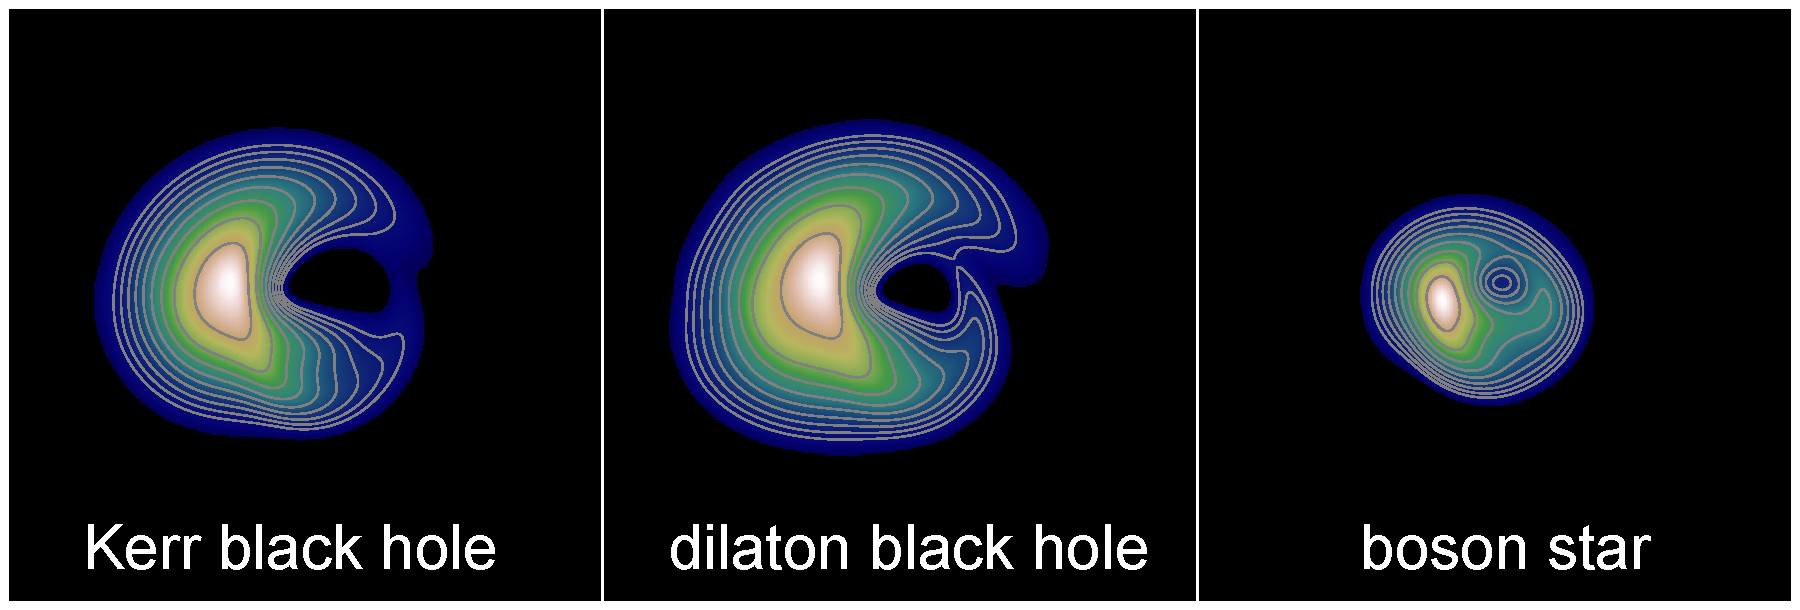
\includegraphics[width=0.88\linewidth,height=0.48\textheight,keepaspectratio]{../figs/pdf/en/fig-07-15.pdf}

% DOCX paragraph 1116
\caption{\emph{Comparison of the images at 230 GHz of three compact objects with the
same mass and subject to the same accretion processes. From left to right: a Kerr black
hole}\index{black hole!Kerr}\emph{, a dilaton black hole, and a boson
star}\index{boson star}\emph{. © C. Fromm/Y. Mizuno/H. Olivares/Z. Younsi/LR.}}\label{fig:07-15}
\end{figure}

% DOCX paragraph 1118
The beauty of Figure \ref{fig:07-15} is that it doesn't need much explanation. It is quite clear
that, while it is possible to notice differences between either of the black holes (left
or central panel) and the boson star\index{boson star} (right panel), this is not true
when comparing the two black holes. In essence, our research has led us to conclude that
it is currently possible to distinguish a black hole from a boson star. A boson star
shows a much smaller shadow\index{shadow (black hole)} than a black hole of the same mass (a
similar behaviour is to be expected for a wormhole, i.e., a smaller shadow for the same
mass). Furthermore, given the fairly tight constraints on the mass of
M87*\index{M87*}, which do not allow the size of the measured shadow to vary too
much, a boson star can be excluded, at least in the model considered so far, from being
compatible with the EHT image. At the same time, given the current quality of the image
of M87*, it is not possible to distinguish with sufficient certainty a Kerr black
hole\index{black hole!Kerr} from a dilaton black hole, even though their images are slightly
different. This explains why this chapter has the title ``The First Image Of A Black
Hole'' and not ``The First Image Of An Einsteinian Black Hole''. At present, we are not
able to distinguish an Einsteinian black hole from one in a dilatonic theory and
probably also from those predicted in many other theories.

% DOCX paragraph 1119
It is possible, and perhaps even likely, that these conclusions will continue to hold
until VLBI observations at much higher resolution are carried out. However, it is also
very likely that new and repeated observations, as are expected in the coming years,
will overcome some of the degeneracies in Figure \ref{fig:07-14}. The simulations clearly show that
the variability\index{variability} in the accretion rate is different in different black
holes, so comparing images taken at varying times can be decisive in breaking the
degeneracy\index{degeneracy!intepretation} now present when comparing only two static images. Once
again, the images taken so far of M87*\index{M87*} should be considered simply as
the first ones; numerous questions remain, which may be answered as new measurements are
carried out.

% DOCX paragraph 1120
I want to end this chapter, dedicated to the first image of a black hole, with a general
consideration. We have already mentioned how the EHT observations have marked a
technological revolution and enormously enriched our understanding of astrophysics and
gravitational physics. In particular, at least two scientific results, generated by the
EHT observations and their theoretical interpretation, are unanimously recognised as the
most relevant. The first is that they have provided evidence, beyond any reasonable
doubt, that there is an accreting supermassive black hole at the centre of galaxy M87.
Since M87 is not a galaxy with peculiar characteristics, by induction, these
observations tell us that every galaxy should have a supermassive black hole at its
centre. It is a hypothesis as old as the first observations of galaxies and black holes
and, remarkably, only confirmed in 2019. Even more important, perhaps, is that the
confirmation of this hypothesis is essential for our current understanding of the
formation of large-scale structures of the universe.

% DOCX paragraph 1121
The second universally recognised contribution of the EHT observations is that they
provided evidence of an essential property of the black-hole solution in general
relativity: its simplicity! It is indeed extraordinary that an object like
M87*\index{M87*}, with a mass of a few billion solar masses, has exactly the same
properties as an object whose mass is a hundred million times smaller, such as the black
holes revealed by the LIGO/Virgo\index{LIGO}\index{Virgo}
gravitational-wave detectors\index{gravitational waves!detectors}. The simple scalability with mass of
black-hole behaviour that we have encountered with the no-hair theorem is a precise
prediction of general relativity. The EHT and LIGO/Virgo observations are so beautifully
complementary; the reason is that they are both necessary to explore the concept of
black holes at the largest and the smallest scales at which they are expected to exist.

% DOCX paragraph 1122
I would add one final consideration that reflects a very personal view: the most
profound relevance of the EHT observations has to be sought elsewhere. What I find most
valuable about the first image of a black hole is that it has transformed the event
horizon\index{event horizon} from a ``mathematical concept'' into a ``physical object''.
In other words, the observations have shown that it is now possible to carry out
experimental tests on what was previously only a concept and, as such, subject to a
variety of different views. Paraphrasing Galileo, these observations, and all those that
follow, essentially allow us to stop ``{[}arguing{]} about the greatest issues without
obtaining any truth''. It is now possible to use actual observations to compare
different and equally plausible theories and thus accept those compatible with the
observations and reject those that are not. The possibility of carrying out this trivial
but essential step in the scientific method\index{scientific method} has been denied us so
far. Therefore, the EHT observations have ultimately provided the simplest and most
important tool for a scientist: the possibility to arrive at truths. In this, I
recognise the greatest value of the M87*\index{M87*} observations.
